\documentclass[xcolor={table}]{beamer}
\usepackage{fleqn}
\usepackage{graphicx}
\usepackage{coordsys} %for \numbline commander

%Setup appearance:
\usetheme{Darmstadt}
\usefonttheme[onlylarge]{structurebold}
\setbeamerfont*{frametitle}{size=\normalsize,series=\bfseries}
\setbeamertemplate{navigation symbols}{}
\setbeamertemplate{bibliography item}{[\theenumiv]}

% Standard packages
\usepackage[english]{babel}
\usepackage[latin1]{inputenc}
\usepackage{times}
\usepackage[T1]{fontenc}
\usepackage{multirow}
\usepackage{subfigure}
\usepackage{pbox}
\usepackage{arydshln}
\usepackage{pifont}
\usepackage{cancel}
\usepackage{rotating} % for sideways headings

% Source Code packages
\usepackage{algorithm2e}
\usepackage{algorithmic}

\DeclareSymbolFont{extraup}{U}{zavm}{m}{n}
\DeclareMathSymbol{\varclub}{\mathalpha}{extraup}{84}
\DeclareMathSymbol{\varspade}{\mathalpha}{extraup}{85}
\DeclareMathSymbol{\varheart}{\mathalpha}{extraup}{86}
\DeclareMathSymbol{\vardiamond}{\mathalpha}{extraup}{87}

%%% This section command that adds a big page with section dividers
\usepackage{xifthen}% provides \isempty test
\newcommand{\SectionSlide}[2][]{
	\ifthenelse{\isempty{#1}}
		{\section{#2}\begin{frame} \begin{center}\begin{huge}#2\end{huge}\end{center}\end{frame}}
		{\section[#1]{#2}\begin{frame} \begin{center}\begin{huge}#2\end{huge}\end{center}\end{frame}}
}
%Extends the section slide to to include a shortened section title for the navigation bar as a second parameter
\newcommand{\SectionSlideShortHeader}[3][]{
	\ifthenelse{\isempty{#1}}
		{\section[#3]{#2}\begin{frame} \begin{center}\begin{huge}#2\end{huge}\end{center}\end{frame}}
		{\section[#1]{#2}\begin{frame} \begin{center}\begin{huge}#3\end{huge}\end{center}\end{frame}}
}

\newcommand{\refer}[1]{\footnote{#1}}
\newcommand{\GW}{\text{\textit{Guess-Who~}}}
\newcommand{\keyword}[1]{\alert{\textbf{#1}}\index{#1}}
\newcommand{\firstkeyword}[1]{\textbf{#1}\index{#1}}
\newcommand{\indexkeyword}[1]{\alert{\textbf{#1}\index{#1}}}
\newcommand{\featN}[1]{\textsc{#1}}
\newcommand{\featL}[1]{\textit{'#1'}}
 \newcommand{\ourRef}[1]{\ref{#1} $^{\text{\tiny[\pageref{#1}]}}$}
 \newcommand{\ourEqRef}[1]{\eqref{#1}$^{\text{\tiny[\pageref{#1}]}}$}
  
\DeclareMathOperator*{\argmax}{argmax}
\DeclareMathOperator*{\argmin}{argmin}

\title{Data Exploration\\Sections $3.1, 3.2, 3.3, 3.4$}
	\author{John D. Kelleher and Brian Mac Namee and Aoife D'Arcy}
	\institute{}
	\date{}
	
\begin{document}
\begin{frame}
	\titlepage
\end{frame}
\begin{frame}
	 \tableofcontents
\end{frame}

\SectionSlide{The Data Quality Report}

 \begin{frame} 
 \begin{itemize}
\item A data quality report includes tabular reports that describe the characteristics of each feature in an ABT using standard statistical measures of \keyword{central tendency} and \keyword{variation}. 
\item The tabular reports are accompanied by data visualizations:
 \begin{itemize}
\item A \indexkeyword{histogram} for each continuous feature in an ABT. 
\item A \indexkeyword{bar plot} for each categorical feature in an ABT.
\end{itemize}
\end{itemize}
\end{frame} 

 \begin{frame} 
\begin{table}[tb]
\caption{The structures of the tables included in a data quality report to describe (a) continuous features and (b) categorical features.}
\label{tab:dataQuality}
\centering
\begin{tiny}
\subtable[Continuous Features]{\label{tab:dataQualityCont}\resizebox{\columnwidth}{!}{\begin{tabular}{  l  c  c  c c  c c c c c c }
\hline
~	 & ~ & \% & ~ & ~	 & $1^{st}$	& ~ & ~ & $3^{rd}$  & ~  & Std.  \\
Feature	 & Count & Miss. & Card. & Min.	 & Qrt.	& Mean & Median & Qrt.  & Max.  & Dev.  \\
\hline
------ & ------ & ------ & ------ & ------ & ------ & ------ & ------ & ------ & ------ & ------ \\
------ & ------ & ------ & ------ & ------ & ------ & ------ & ------ & ------ & ------ & ------ \\
------ & ------ & ------ & ------ & ------ & ------ & ------ & ------ & ------ & ------ & ------ \\
\hline
\end{tabular}}}

\subtable[Categorical Features]{\label{tab:dataQualityCat}\resizebox{\columnwidth}{!}{\begin{tabular}{  l  c  c  c c c c c c c}
\hline
~ & ~ & ~ & ~	 & ~	 & ~ & ~ & ~	& $2^{nd}$ & $2^{nd}$  \\
~ & ~ & \% & ~	 & ~	 & Mode & Mode & $2^{nd}$	& Mode & Mode  \\
Feature	& Count & Miss. & Card. & Mode	 & Freq. & \% & Mode	& Freq. & \%  \\
\hline
------ & ------ & ------ & ------ & ------ & ------ & ------ & ------ & ------ & ------ \\
------ & ------ & ------ & ------ & ------ & ------ & ------ & ------ & ------ & ------ \\
------ & ------ & ------ & ------ & ------ & ------ & ------ & ------ & ------ & ------ \\
\hline
\end{tabular}}}
\end{tiny}
\end{table}
\end{frame} 


\subsection{Case Study: Motor Insurance Fraud}

\begin{frame}[plain]
\begin{block}{Case Study: Motor Insurance Fraud}
The following slides show a portion of the ABT that has been developed for the motor insurance claims fraud detection.

~\\

A portion of the ABT developed for this solution is shown first.
\end{block}
\end{frame}



 \begin{frame} [plain]
\begin{table}[tb]
\caption{Portions of the ABT for the motor insurance claims fraud detection problem.}
\label{table:fraudDetectionData}
\centering
\begin{tiny}
\resizebox{\textwidth}{!}{
\begin{tabular}{ r c r c c c c r r c c c r c}
\hline
~ & ~ & ~ & ~ & ~ & ~	& ~ & ~ & ~ & ~	&	\featN{Num}	&	\featN{\%}	&	\featN{Claim}	 &	~	\\
~	&	~	&	~	&	\featN{Marital}	&	\featN{Num}	&	\featN{Injury}	&	\featN{Hospital}	&	\featN{Claim}	&	\featN{Total}	&	\featN{Num}	&	\featN{Soft}	&	\featN{Soft}	&	\featN{Amt}	 &	\featN{Fraud}	\\
\featN{ID}	&	\featN{Type}	&	\featN{Inc.}	&	\featN{Status} &	\featN{Clmnts.}	&	\featN{Type}	&	\featN{Stay}	&	\featN{Amnt.}	&	\featN{Claimed}	&	\featN{Claims} &	\featN{Tiss.}	&	\featN{Tiss.}	&	\featN{Rcvd.}	 &	\featN{Flag}	\\
\hline
1	&	CI	&	0	&		&	2	&	Soft Tissue	&	No	&	1,625	&	3250	&	2	&	2	&	1.0	&	0	&	1	\\
2	&	CI	&	0	&		&	2	&	Back	&	Yes	&	15,028	&	60,112	&	1	&		&	0	&	15,028	&	0	\\
3	&	CI	&	54,613	&	Married	&	1	&	Broken Limb	&	No	&	-99,999	&	0	&	0	&	0	&	0	&	572	&	0	\\
4	&	CI	&	0	&		&	4	&	Broken Limb	&	Yes	&	5,097	&	11,661	&	1	&	1	&	1.0 	&	7,864	&	0	\\
5	&	CI	&	0	&		&	4	&	Soft Tissue	&	No	&	8869	&	0	&	0	&	0	&	0	&	0	&	1	\\
6	&	CI	&	0	&		&	1	&	Broken Limb	&	Yes	&	17,480	&	0	&	0	&	0	&	0	&	17,480	&	0	\\
7	&	CI	&	52,567	&	Single	&	3	&	Broken Limb	&	No	&	3,017	&	18,102	&	2	&	1	&	0.5 	&	0	&	1	\\
8	&	CI	&	0	&		&	2	&	Back	&	Yes	&	7463	&	0	&	0	&	0	&	0	&	7,463	&	0	\\
9	&	CI	&	0	&		&	1	&	Soft Tissue	&	No	&	2,067	&	0	&	0	&	0	&	0	&	2,067	&	0	\\
10	&	CI	&	42,300	&	Married	&	4	&	Back	&	No	&	2,260	&	0	&	0	&	0	&	0	&	2,260	&	0	\\
\multicolumn{5}{c}{$\vdots$} & \multicolumn{4}{c}{$\vdots$} & \multicolumn{5}{c}{$\vdots$} \\
300	&	CI	&	0	&		&	2	&	Broken Limb	&	No	&	2,244	&	0	&	0	&	0	&	0	&	2,244	&	0	\\
301	&	CI	&	0	&		&	1	&	Broken Limb	&	No	&	1,627	&	92,283	&	3	&	0	&	0	&	1,627	&	0	\\
302	&	CI	&	0	&		&	3	&	Serious	&	Yes	&	270,200	&	0	&	0	&	0	&	0	&	270,200	&	0	\\
303	&	CI	&	0	&		&	1	&	Soft Tissue	&	No	&	7,668	&	92,806	&	3	&	0	&	0	&	7,668	&	0	\\
304	&	CI	&	46,365	&	Married	&	1	&	Back	&	No	&	3,217	&	0	&	0	&		&	0	&	1,653	&	0	\\
\multicolumn{5}{c}{$\vdots$} & \multicolumn{4}{c}{$\vdots$} & \multicolumn{5}{c}{$\vdots$} \\
458	&	CI	&	48,176	&	Married	&	3	&	Soft Tissue	&	Yes	&	4,653	&	8,203	&	1	&	0	&	0	&	4,653	&	0	\\
459	&	CI	&	0	&		&	1	&	Soft Tissue	&	Yes	&	881	&	51,245	&	3	&	0	&	0	&	0	&	1	\\
460	&	CI	&	0	&		&	3	&	Back	&	No	&	8,688	&	729,792	&	56	&	5	&	0.08	&	8,688	&	0	\\
461	&	CI	&	47,371	&	Divorced	&	1	&	Broken Limb	&	Yes	&	3,194	&	11,668	&	1	&	0	&	0	&	3,194	&	0	\\
462	&	CI	&	0	&		&	1	&	Soft Tissue	&	No	&	6,821	&	0	&	0	&	0	&	0	&	0	&	1	\\
\multicolumn{5}{c}{$\vdots$} & \multicolumn{4}{c}{$\vdots$} & \multicolumn{5}{c}{$\vdots$} \\
491	&	CI	&	40,204	&	Single	&	1	&	Back	&	No	&	75,748	&	11,116	&	1	&	0	&	0	&	0	&	1	\\
492	&	CI	&	0	&		&	1	&	Broken Limb	&	No	&	6,172	&	6,041	&	1	&		&	0	&	6,172	&	0	\\
493	&	CI	&	0	&		&	1	&	Soft Tissue	&	Yes	&	2,569	&	20,055	&	1	&	0	&	0	&	2,569	&	0	\\
494	&	CI	&	31,951	&	Married	&	1	&	Broken Limb	&	No	&	5,227	&	22,095	&	1	&	0	&	0	&	5,227	&	0	\\
495	&	CI	&	0	&		&	2	&	Back	&	No	&	3,813	&	9,882	&	3	&	0	&	0	&	0	&	1	\\
496	&	CI	&	0	&		&	1	&	Soft Tissue	&	No	&	2,118	&	0	&	0	&	0	&	0	&	0	&	1	\\
497	&	CI	&	29,280	&	Married	&	4	&	Broken Limb	&	Yes	&	3,199	&	0	&	0	&	0	&	0	&	0	&	1	\\
498	&	CI	&	0	&		&	1	&	Broken Limb	&	Yes	&	32,469	&	0	&	0	&	0	&	0	&	16,763	&	0	\\
499	&	CI	&	46,683	&	Married	&	1	&	Broken Limb	&	No	&	179,448	&	0	&	0	&		&	0	&	179,448	&	0	\\
500	&	CI	&	0	&		&	1	&	Broken Limb	&	No	&	8,259	&	0	&	0	&	0	&	0	&	0	&	1	\\
\hline
\end{tabular}}
\end{tiny}
\end{table}
\end{frame} 



 \begin{frame} [plain]
\begin{table}[tb]
\caption{A data quality report for the motor insurance claims fraud detection ABT}
\centering
\begin{footnotesize}
\subtable[Continuous Features]{\label{table:dataQualityExampleCont}\resizebox{\textwidth}{!}{\begin{tabular}{  l  c  r  c r  r r r r r r}
\hline
~	 & ~ & \% & ~ & ~	 & $1^{st}$	& ~ & ~ & $3^{rd}$  & ~  & Std.  \\
Feature	 & Count & Miss. & Card. & Min	 & Qrt.	& Mean & Median & Qrt.  & Max  & Dev. \\
\hline
\featN{Income} & 500 & 0.0 & 171 & 0.0 & 0.0 & 13,740.0 & 0.0 & 33,918.5 & 71,284.0 & 20,081.5  \\
\featN{Num Claimants} & 500 & 0.0 & 4 & 1.0 & 1.0 & 1.9 & 2 & 3.0 & 4.0 & 1.0 \\
\featN{Claim Amount} & 500 & 0.0 & 493 & -99,999 & 3,322.3 & 16,373.2 & 5,663.0 & 12,245.5 & 270,200.0 & 29,426.3 \\
\featN{Total Claimed} & 500 & 0.0 & 235 & 0.0 & 0.0 & 9,597.2 & 0.0 & 11,282.8 & 729,792.0 & 35,655.7 \\
\featN{Num Claims} & 500 & 0.0 & 7 & 0.0 & 0.0 & 0.8 & 0.0 & 1.0 & 56.0 & 2.7 \\
\featN{Num Soft Tissue} & 500 & 2.0 & 6 & 0.0 & 0.0 & 0.2 & 0.0 & 0.0 & 5.0 & 0.6 \\
\featN{\% Soft Tissue} & 500 & 0.0 & 9 & 0.0 & 0.0 & 0.2 & 0.0 & 0.0 & 2.0 & 0.4 \\
\featN{Amount Received} & 500 & 0.0 & 329 & 0.0 & 0.0 & 13,051.9 & 3,253.5 & 8,191.8 & 295,303.0 & 30,547.2 \\
\featN{Fraud Flag} & 500 & 0.0 & 2 & 0.0 & 0.0 & 0.3 & 0.0 & 1.0 & 1.0  & 0.5 \\
\hline
\end{tabular}}}
\end{footnotesize}
\end{table}
\end{frame} 

 \begin{frame} [plain]
\begin{table}[tb]
\caption{A data quality report for the motor insurance claims fraud detection ABT.}
\label{table:dataQualityExample}
\centering
\begin{footnotesize}
\subtable[Categorical Features]{\label{table:dataQualityExampleCat}\resizebox{\textwidth}{!}{\begin{tabular}{  l  c r c c r r c r r}
\hline
~ & ~ & ~ & ~	 & ~	 & ~ & ~ & ~	& $2^{nd}$ & $2^{nd}$  \\
~ & ~ & \% & ~	 & ~	 & Mode & Mode & $2^{nd}$	& Mode & Mode  \\
Feature	& Count & Miss. & Card. & Mode	 & Freq. & \% & Mode	& Freq. & \% \\
\hline
\featN{Insurance Type} & 500 & 0.0 & 1 & CI & 500 & 1.0 & -- & -- & -- \\
\featN{Marital Status} & 500 & 61.2 & 4 & Married & 99 & 51.0 & Single & 48 & 24.7 \\
\featN{Injury Type} & 500 & 0.0 & 4 & Broken Limb & 177 & 35.4 & Soft Tissue & 172 & 34.4 \\
\featN{Hospital Stay} & 500 & 0.0 & 2 & No & 354 & 70.8 & Yes & 146 & 29.2 \\
\hline
\end{tabular}}}
\end{footnotesize}
\end{table}
\end{frame} 

 \begin{frame} [plain]
\begin{figure}[!thb]
\centering
\subfigure[\scriptsize{\featN{Income}}]{\label{fig:dataQualityPlotExamples3}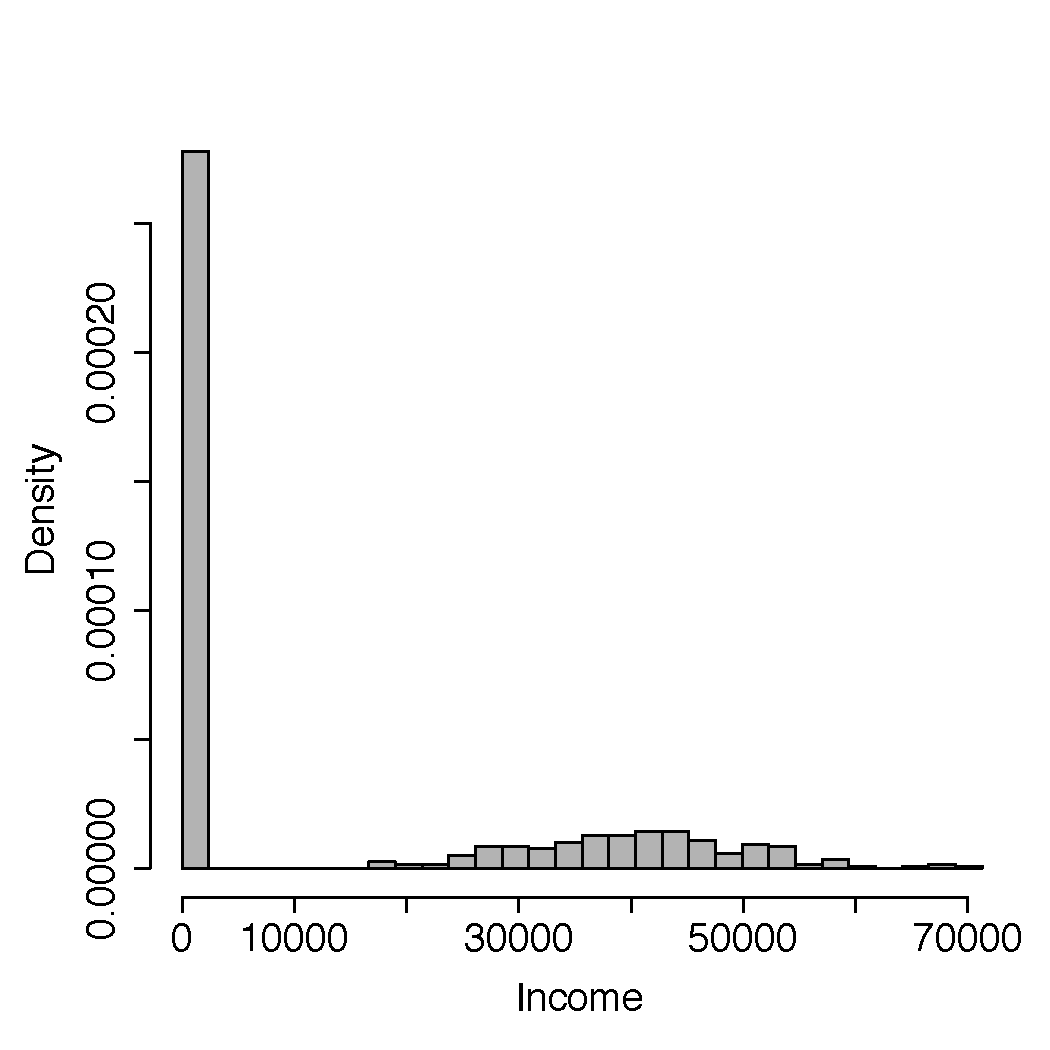
\includegraphics[width=0.3\linewidth]{./images/DataEx_Fraud_Big_Income_of_Policy_Holder_hist_All.pdf}}
\subfigure[\scriptsize{\featN{Num Claimants}}]{\label{fig:dataQualityPlotExamples5}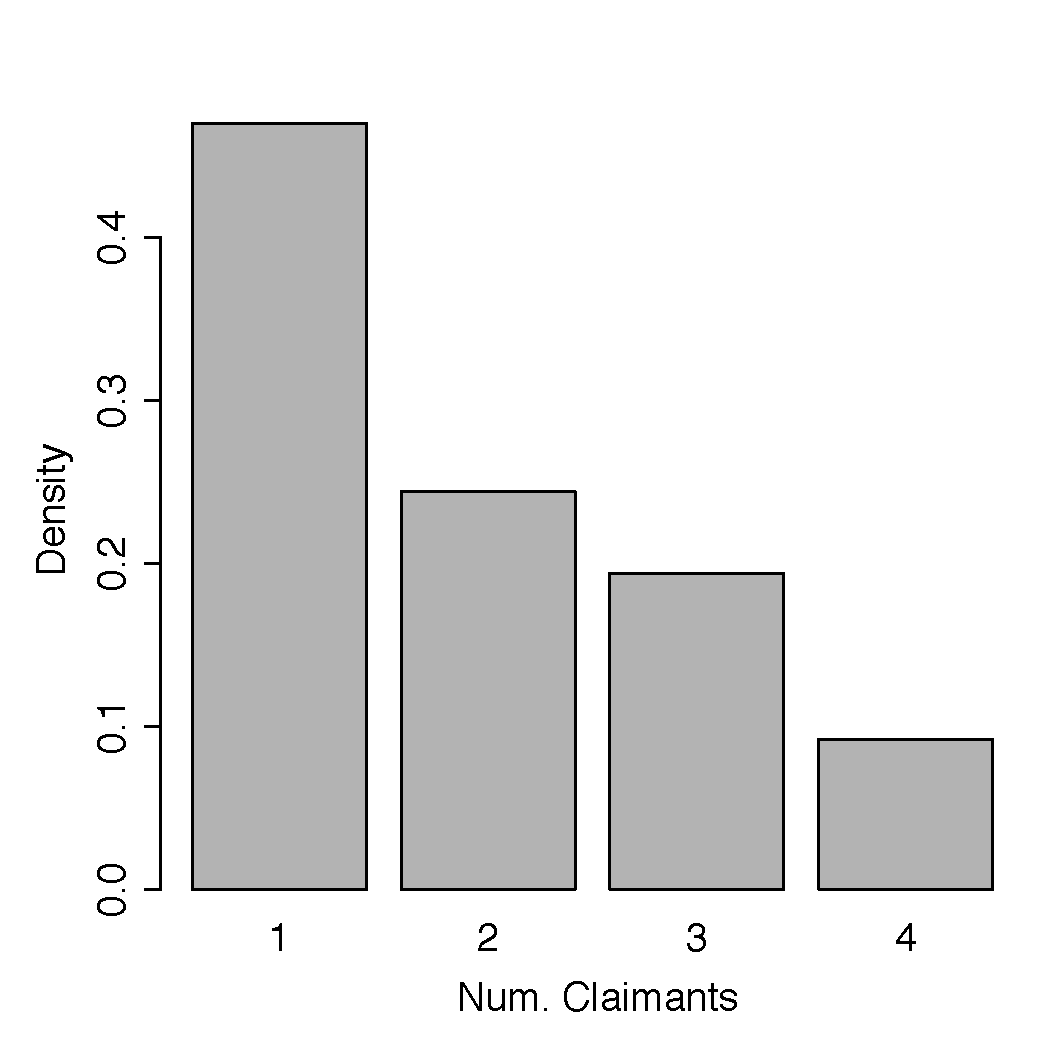
\includegraphics[width=0.3\linewidth]{./images/DataEx_Fraud_Big_Num_Claimants_bar_All.pdf}} \\
\subfigure[\scriptsize{\featN{Claim Amount}}]{\label{fig:dataQualityPlotExamples8}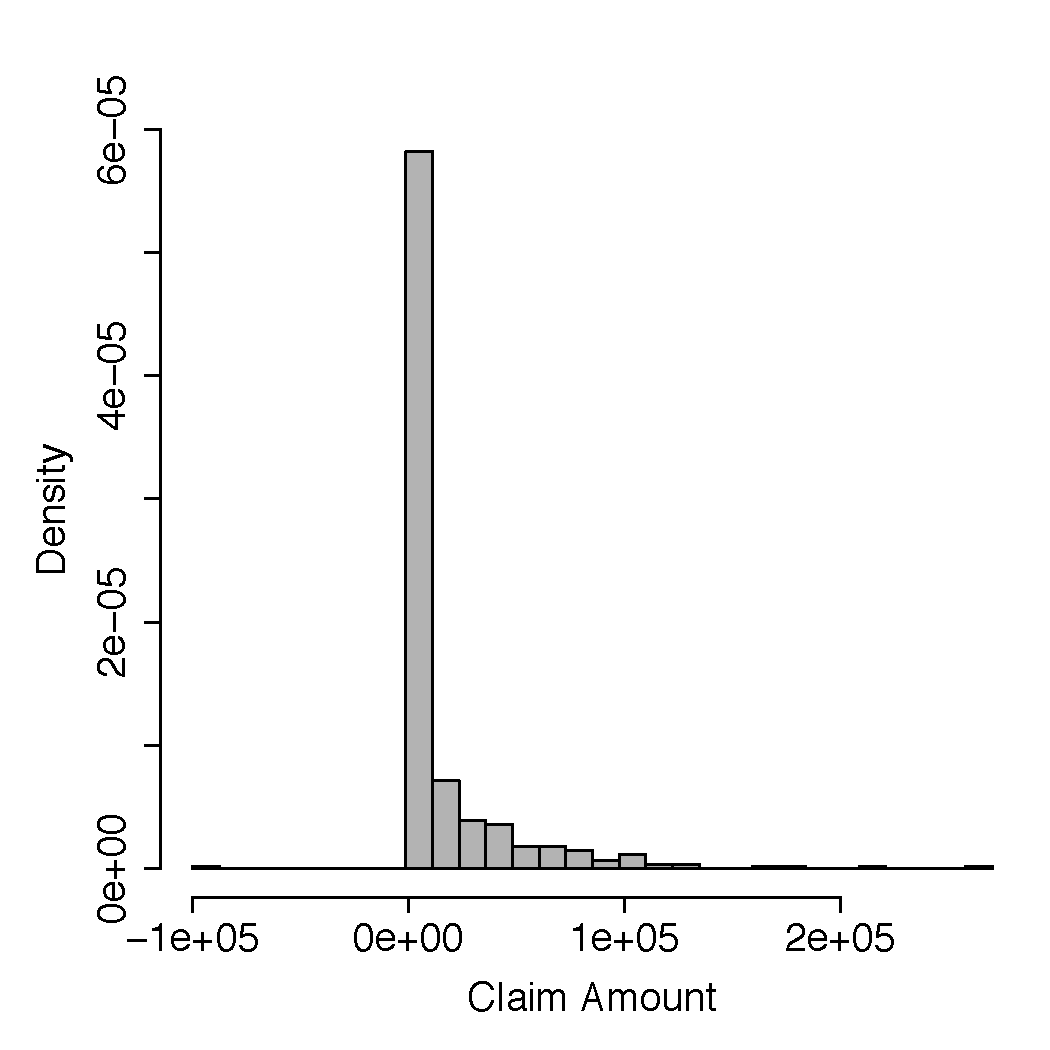
\includegraphics[width=0.3\linewidth]{./images/DataEx_Fraud_Big_Claim_Amount_hist_All.pdf}}
\subfigure[\scriptsize{\featN{Total Claimed}}]{\label{fig:dataQualityPlotExamples9}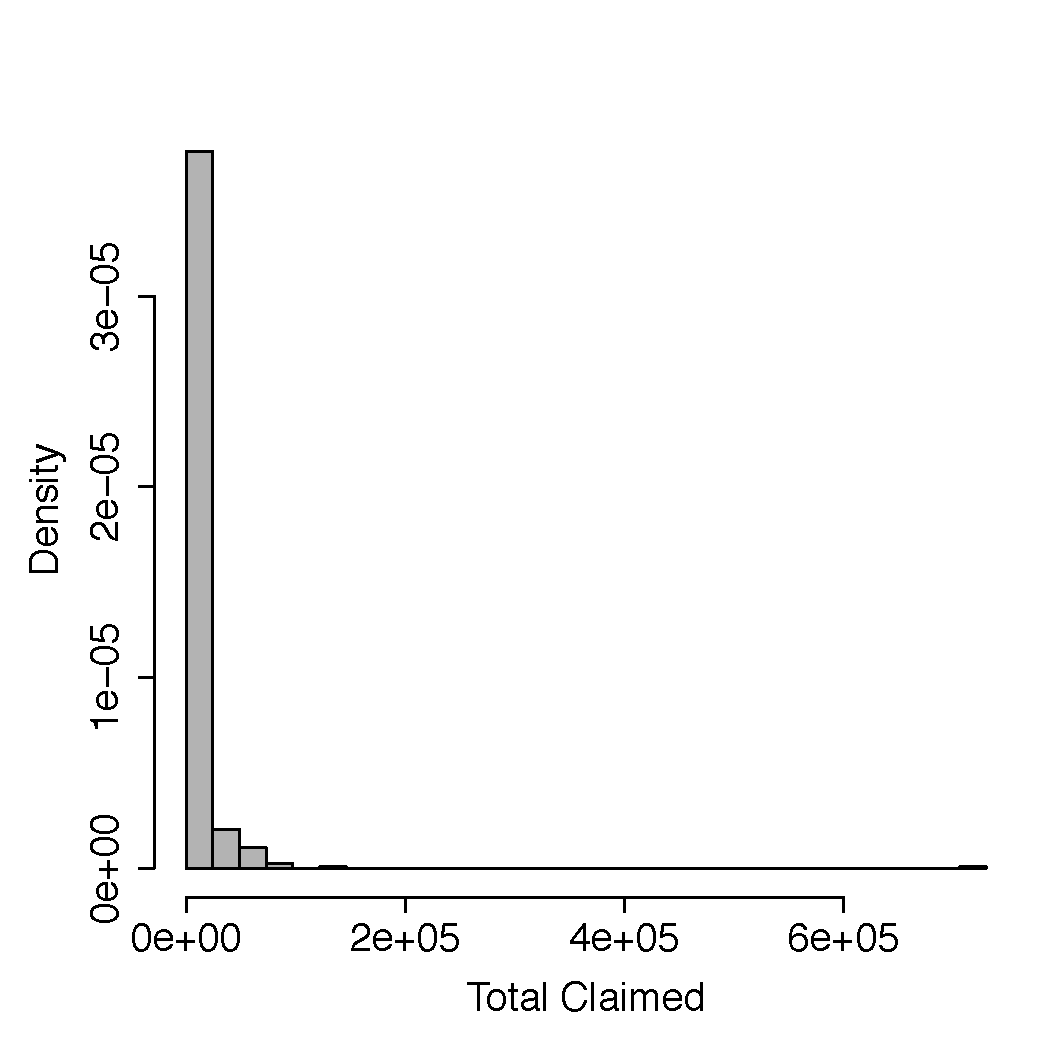
\includegraphics[width=0.3\linewidth]{./images/DataEx_Fraud_Big_Total_Claimed_hist_All.pdf}} 
\caption{Visualizations of the continuous and categorical features in the motor insurance claims fraud detection ABT in Table \ourRef{table:fraudDetectionData}.}
\label{fig:dataQualityPlotExamples}
\end{figure}
\end{frame} 

 \begin{frame} [plain]
\begin{figure}[!thb]
\centering
\subfigure[\scriptsize{\featN{Num Claims}}]{\label{fig:dataQualityPlotExamples10}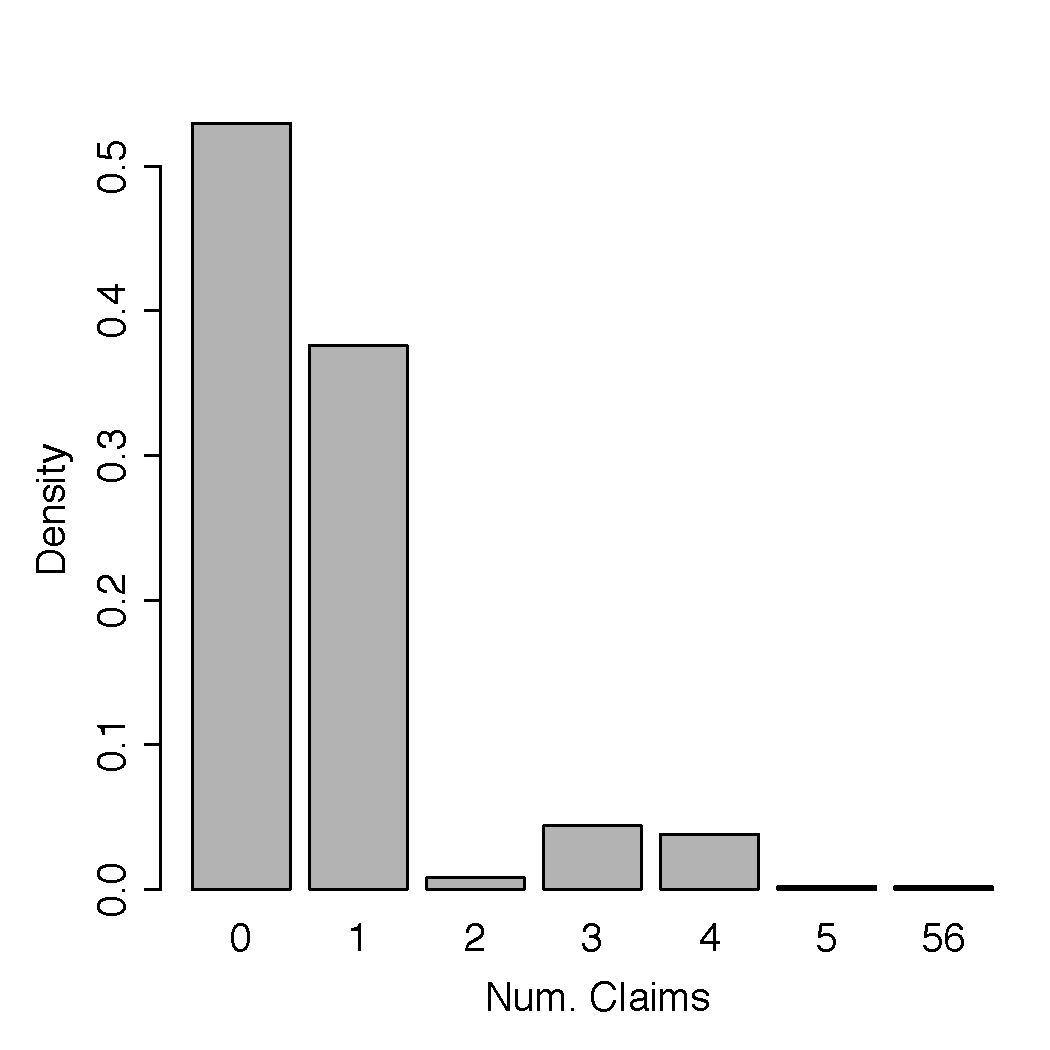
\includegraphics[width=0.3\linewidth]{./images/DataEx_Fraud_Big_Num_Claims_bar_All.pdf}} 
\subfigure[\scriptsize{\featN{Num Soft Tissue}}]{\label{fig:dataQualityPlotExamples11}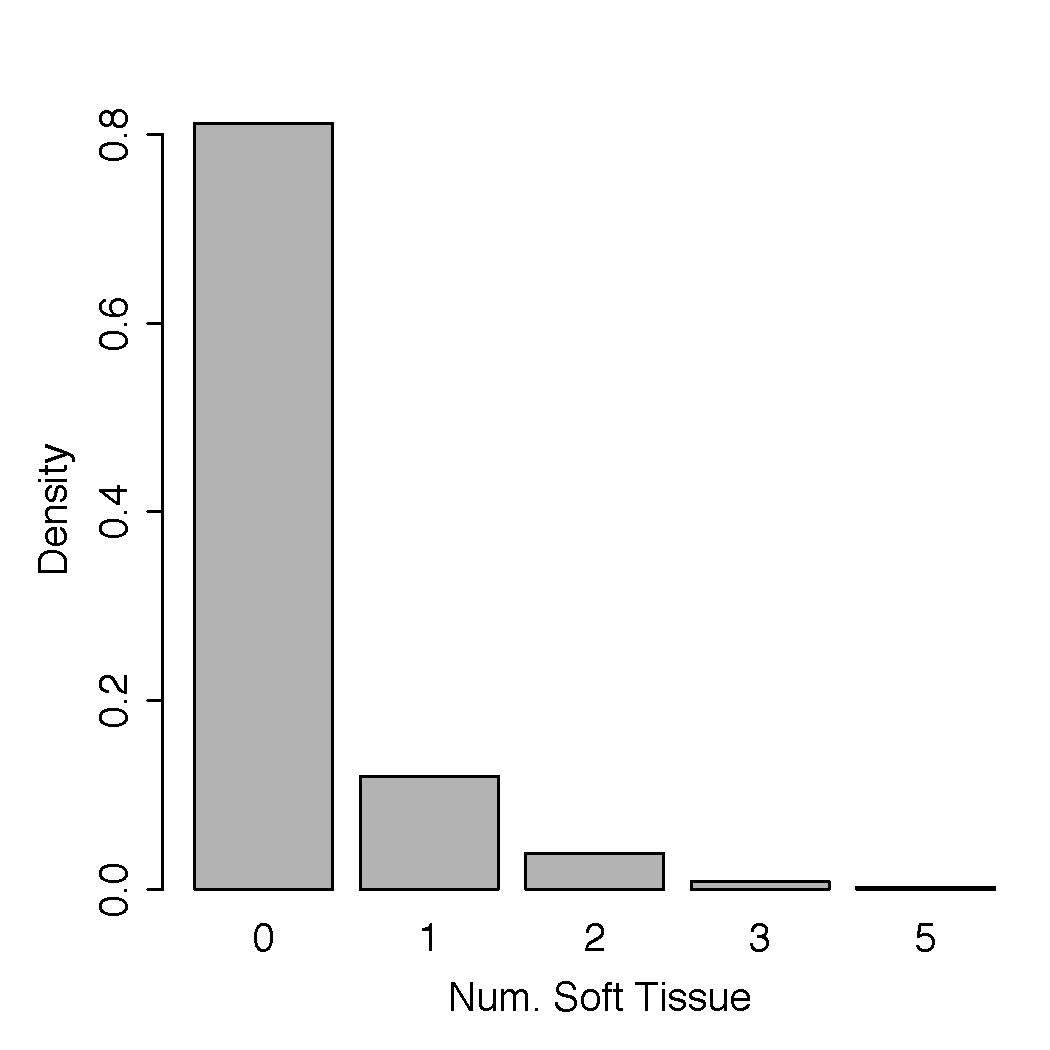
\includegraphics[width=0.3\linewidth]{./images/DataEx_Fraud_Big_Num_Soft_Tissue_bar_All.pdf}}  \\
\subfigure[\scriptsize{\featN{\% Soft Tissue}}]{\label{fig:dataQualityPlotExamples12}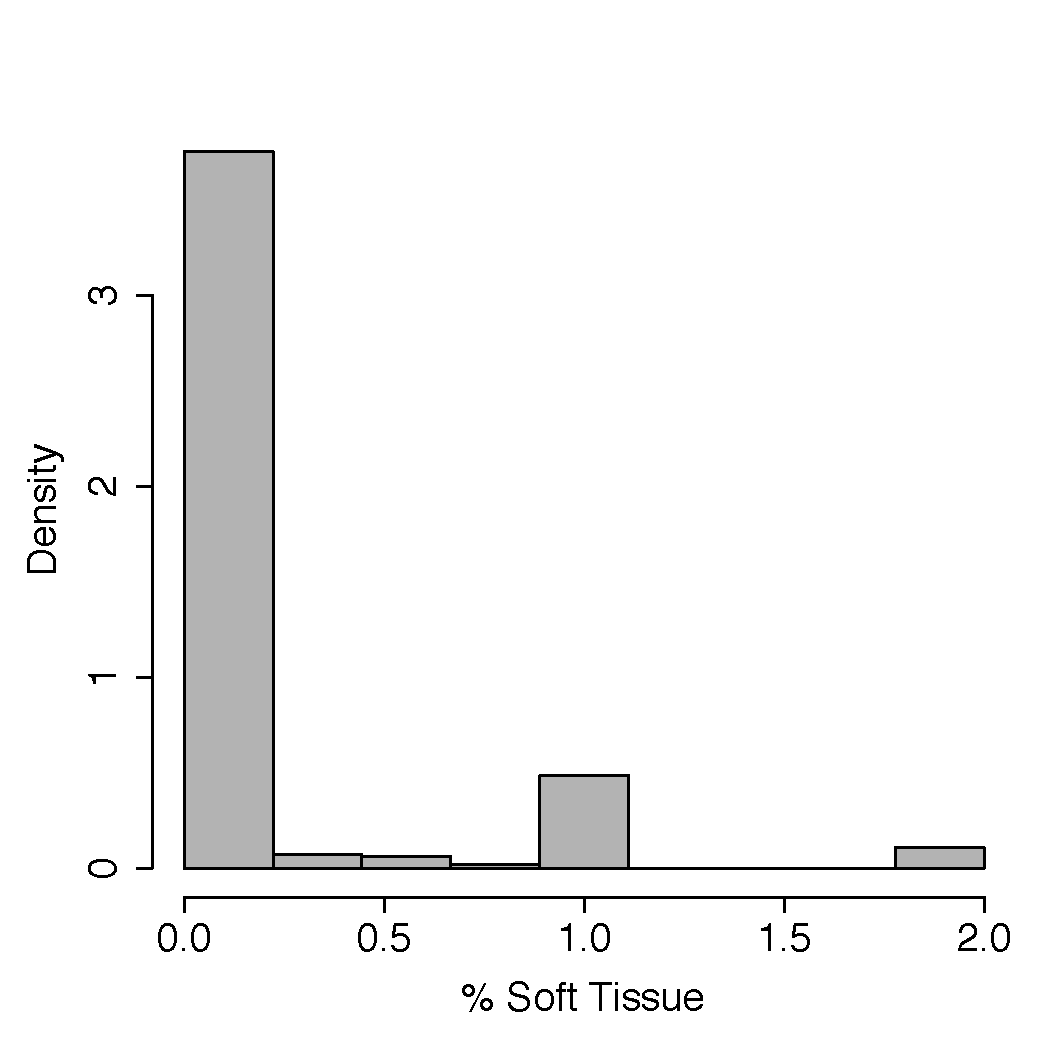
\includegraphics[width=0.3\linewidth]{./images/DataEx_Fraud_Big_X_Soft_Tissue_hist_All.pdf}}
\subfigure[\scriptsize{\featN{Amount Received}}]{\label{fig:dataQualityPlotExamples13}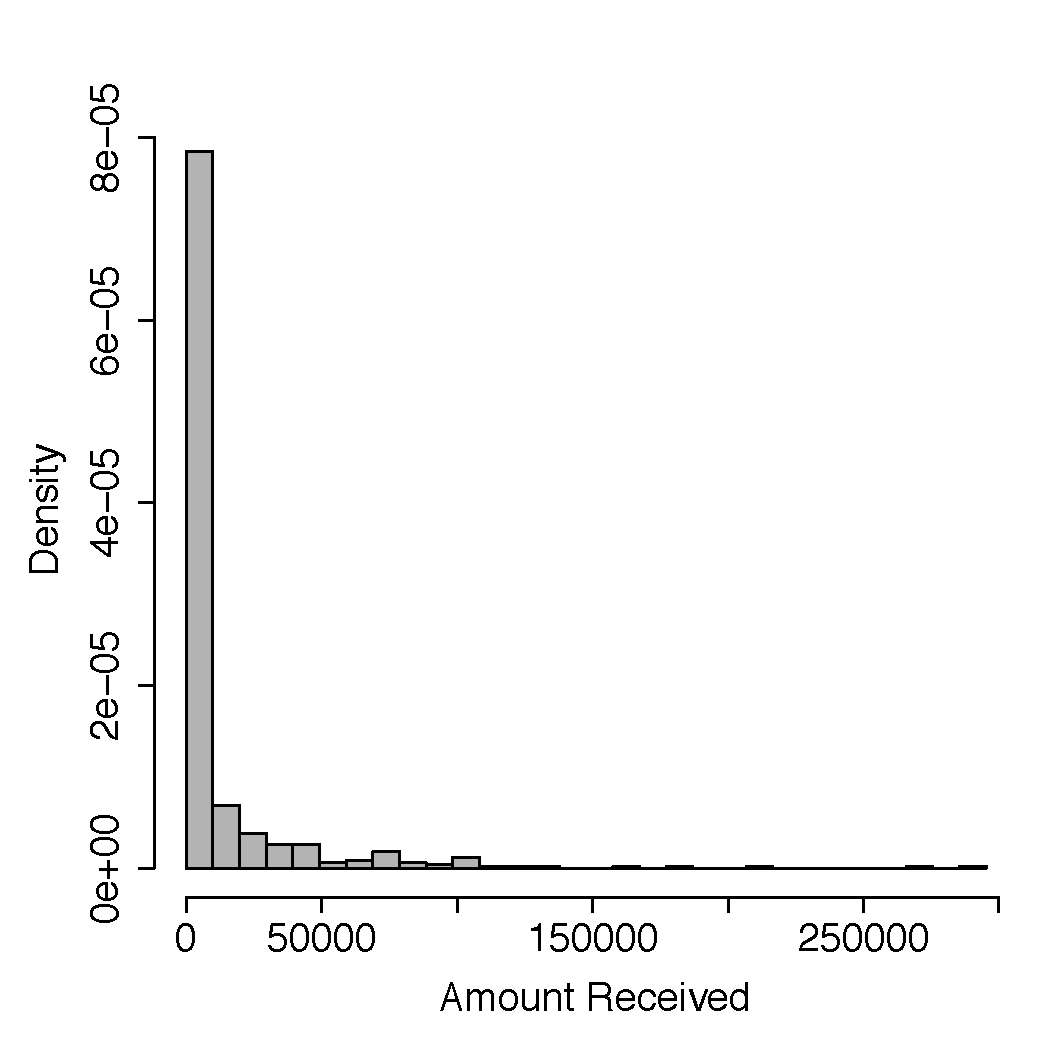
\includegraphics[width=0.3\linewidth]{./images/DataEx_Fraud_Big_Claim_Amount_Received_hist_All.pdf}}
\caption{Visualizations of the continuous and categorical features in the motor insurance claims fraud detection ABT in Table \ourRef{table:fraudDetectionData}.}
\label{fig:dataQualityPlotExamples}
\end{figure}
\end{frame} 

 \begin{frame} [plain]
\begin{figure}[!thb]
\centering
\subfigure[\scriptsize{\featN{Marital Status}}]{\label{fig:dataQualityPlotExamples4}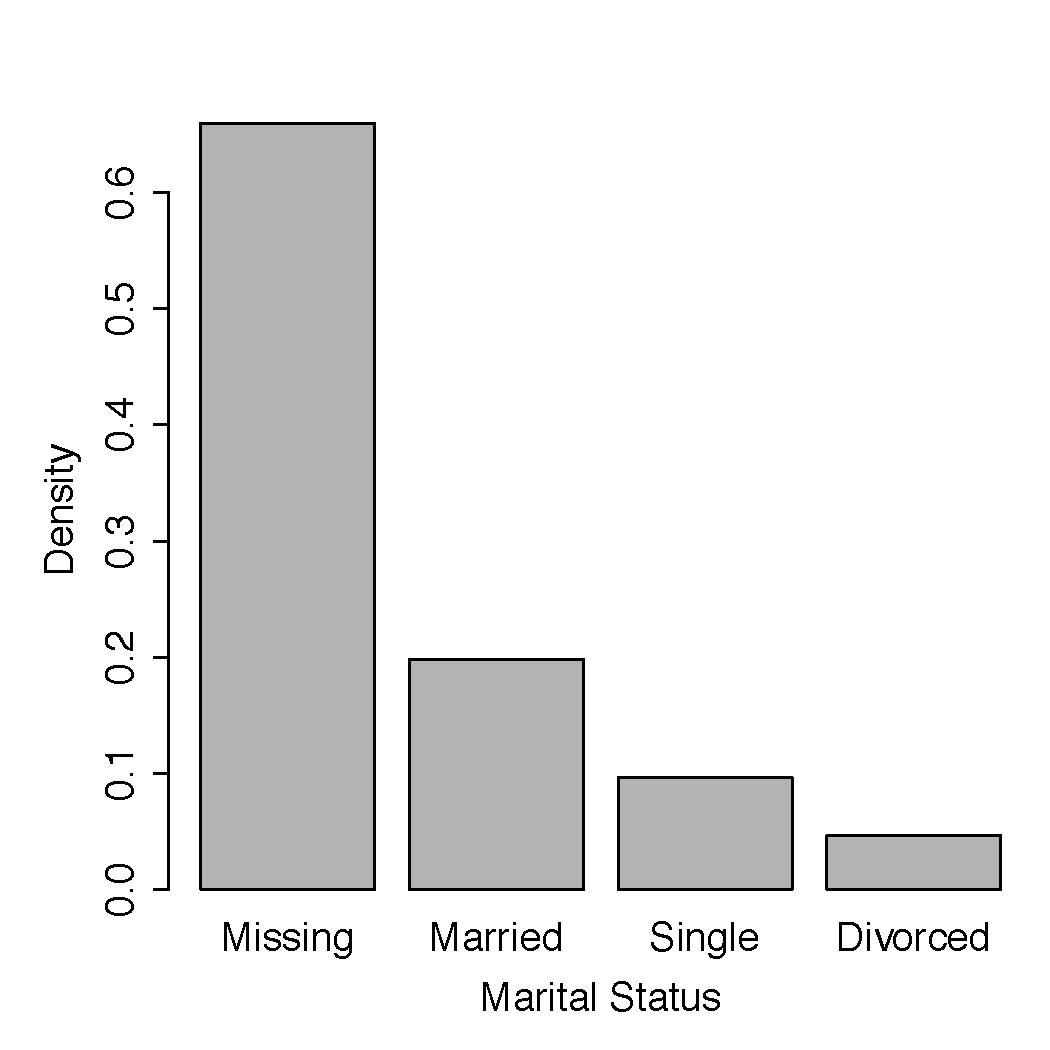
\includegraphics[width=0.3\linewidth]{./images/DataEx_Fraud_Big_Marital_Status_bar_All.pdf}} 
\subfigure[\scriptsize{\featN{Injury Type}}]{\label{fig:dataQualityPlotExamples6}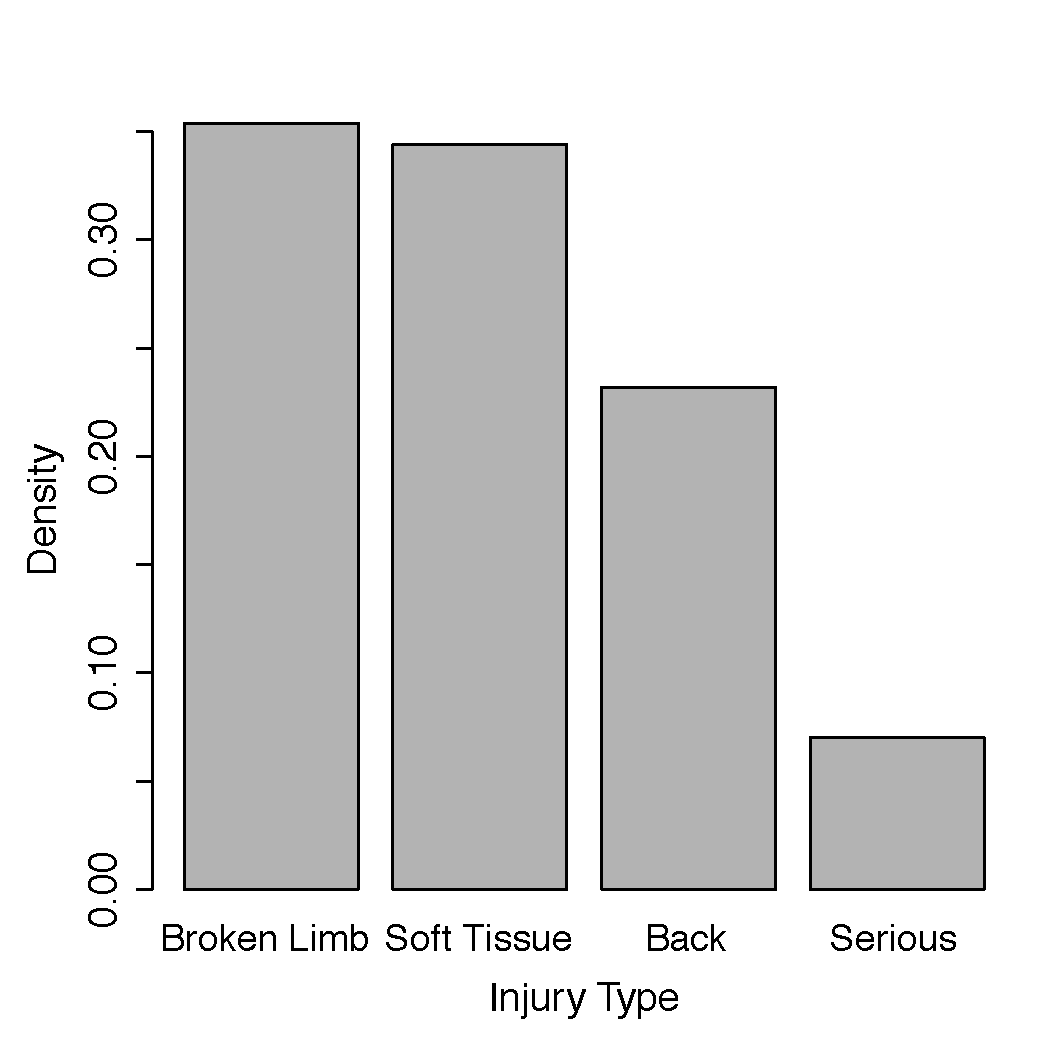
\includegraphics[width=0.3\linewidth]{./images/DataEx_Fraud_Big_Injury_Type_bar_All.pdf}}
\subfigure[\scriptsize{\featN{Hospital Stay}}]{\label{fig:dataQualityPlotExamples7}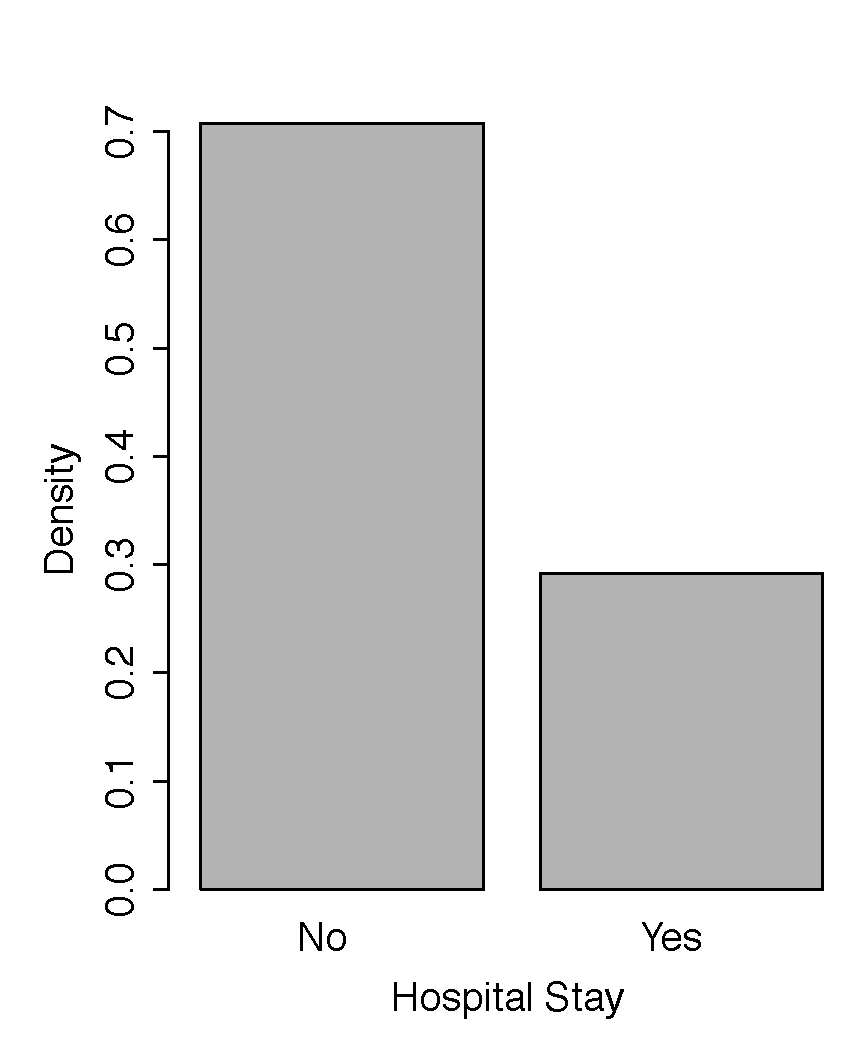
\includegraphics[width=0.25\linewidth]{./images/DataEx_Fraud_Big_Overnight_Hospital_Stay_bar_All.pdf}} 
\caption{Visualizations of the continuous and categorical features in the motor insurance claims fraud detection ABT in Table \ourRef{table:fraudDetectionData}.}
\label{fig:dataQualityPlotExamples}
\end{figure}
\end{frame}

 \begin{frame} [plain]
\begin{figure}[!thb]
\centering
\subfigure[\scriptsize{\featN{Fraud Flag}}]{\label{fig:dataQualityPlotExamples14}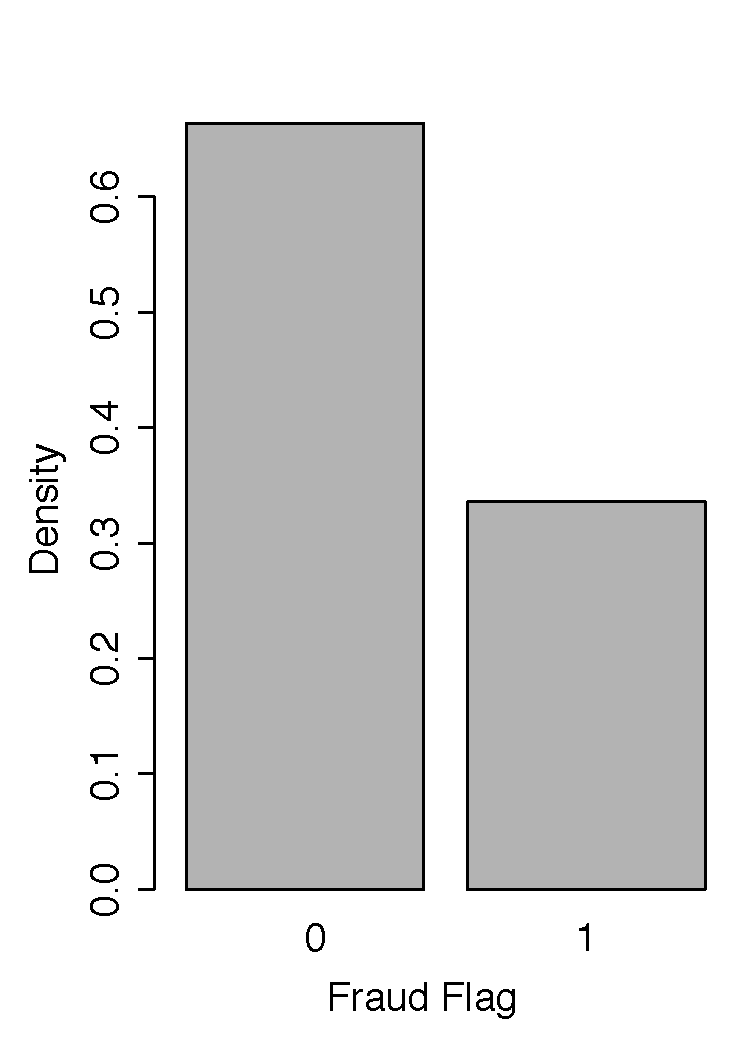
\includegraphics[width=0.25\linewidth]{./images/DataEx_Fraud_Big_Fraud_Flag_bar_All.pdf}} 
\subfigure[\scriptsize{\featN{Insurance Type}}]{\label{fig:dataQualityPlotExamples2}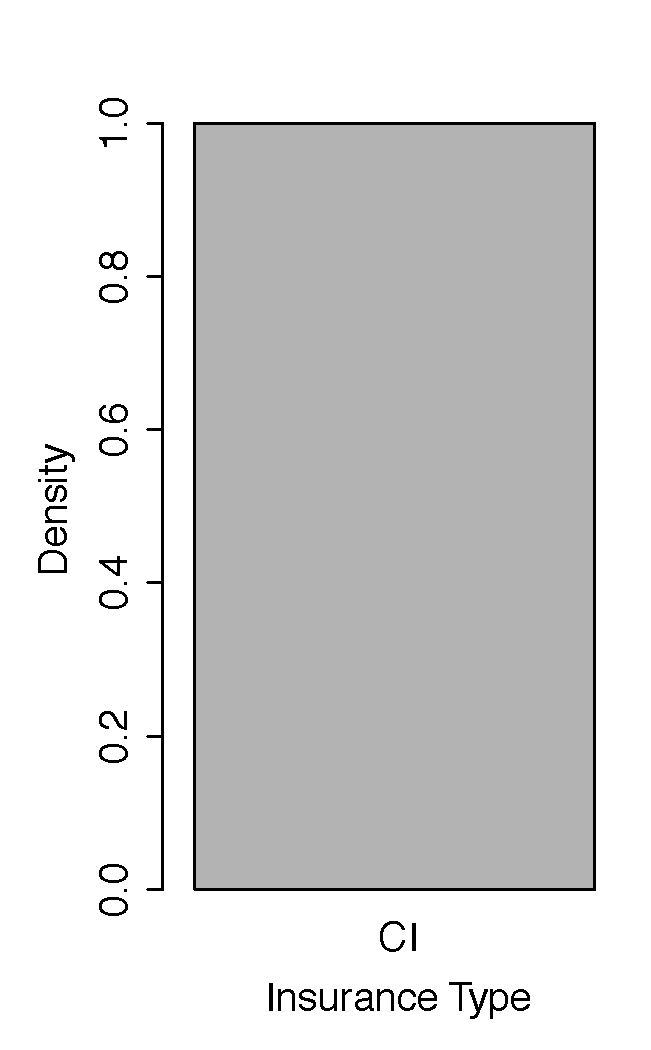
\includegraphics[width=0.21\linewidth]{./images/DataEx_Fraud_Big_Insurance_Type_bar_All.pdf}} 
\caption{Visualizations of the continuous and categorical features in the motor insurance claims fraud detection ABT in Table \ourRef{table:fraudDetectionData}.}
\label{fig:dataQualityPlotExamples}
\end{figure}
\end{frame} 




\SectionSlide{Getting To Know The Data}

 \begin{frame} 
 \begin{itemize} 
 \item For categorical features, we should:
 \begin{itemize} 
 \item Examine the mode, $2^{nd}$ mode, mode \%, and  $2^{nd}$ mode \%  as these tell us the most common levels within these features and will identify if any levels dominate the dataset. 
\end{itemize} 
\item For continuous features we should:
\begin{itemize} 
\item Examine the mean and standard deviation of each feature to get a sense of the central tendency and variation of the values within the dataset for the feature. 
\item Examine the minimum and maximum values to understand the range that is possible for each feature. 
\end{itemize} 
\end{itemize} 
\end{frame} 

\begin{frame}
	\begin{itemize}
		\item When we generate histograms of features there are a number of common, well understood shapes that we should look out for. 
		\end{itemize}
\end{frame}

 \begin{frame} 
\begin{figure}[htb]
\centering
\subfigure[\tiny Uniform]{\label{fig:hist_uniform}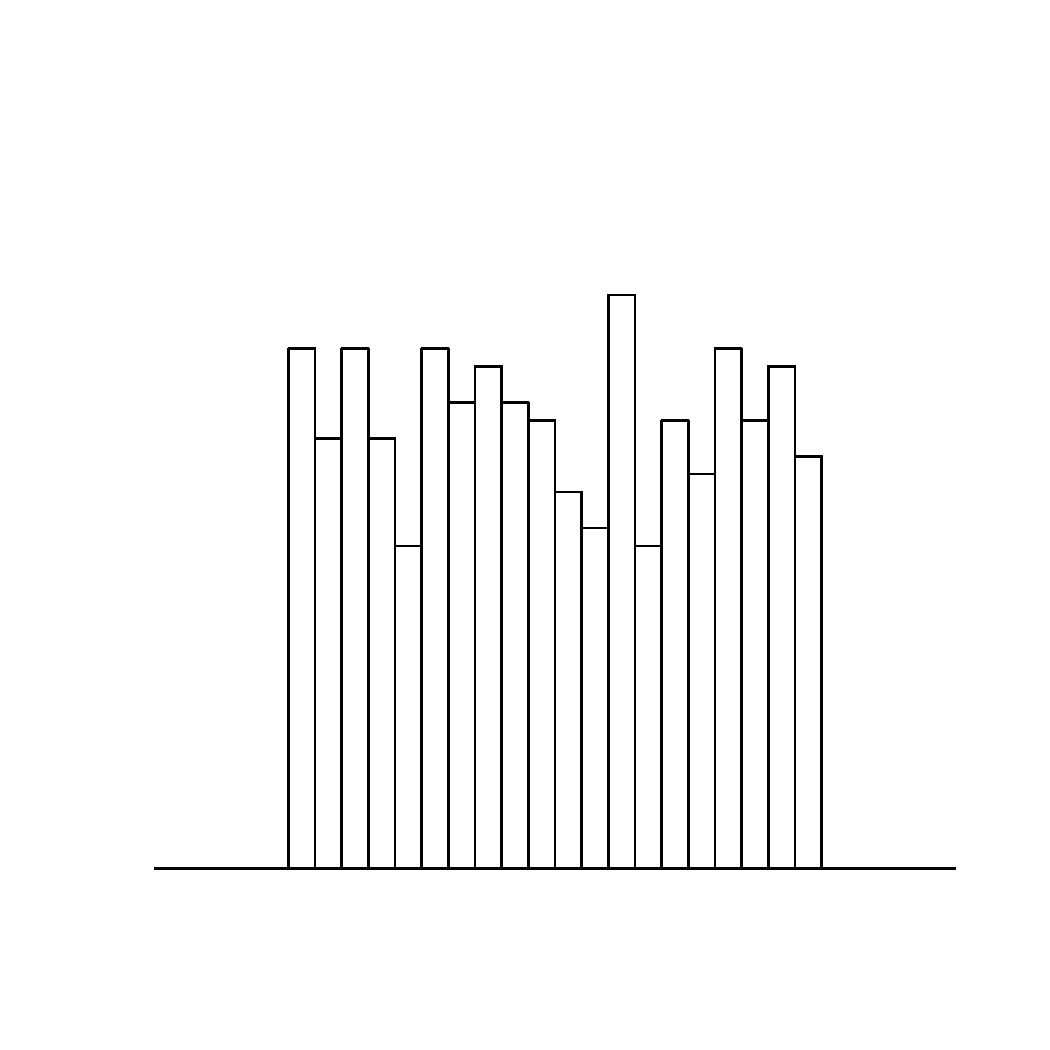
\includegraphics[width=0.32\textwidth]{./images/HistogramShapes_uniform.pdf}} 
\subfigure[\tiny Normal (Unimodal)]{\label{fig:hist_uni}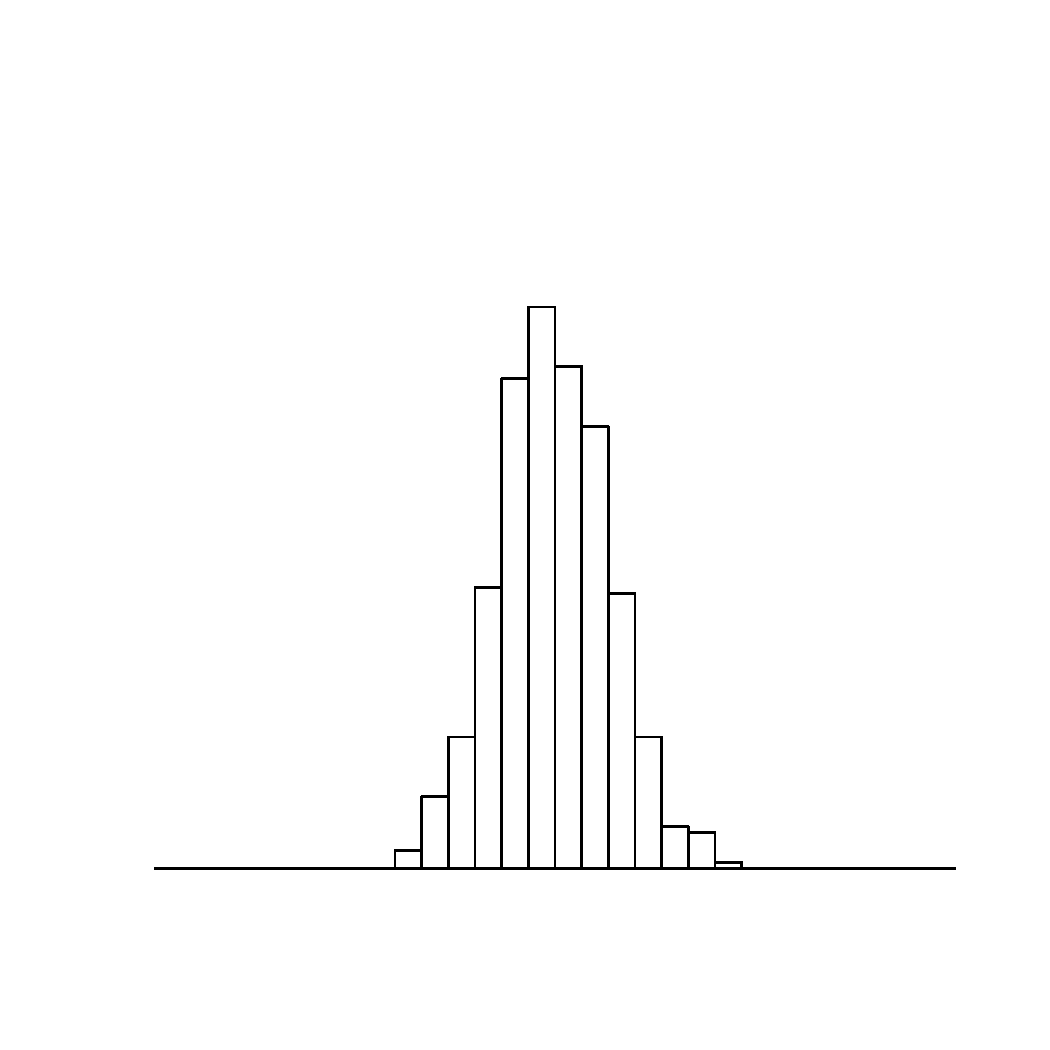
\includegraphics[width=0.32\textwidth]{./images/HistogramShapes_unimodal.pdf}}
\subfigure[\tiny Unimodal (skewed right)]{\label{fig:hist_uni_skewr}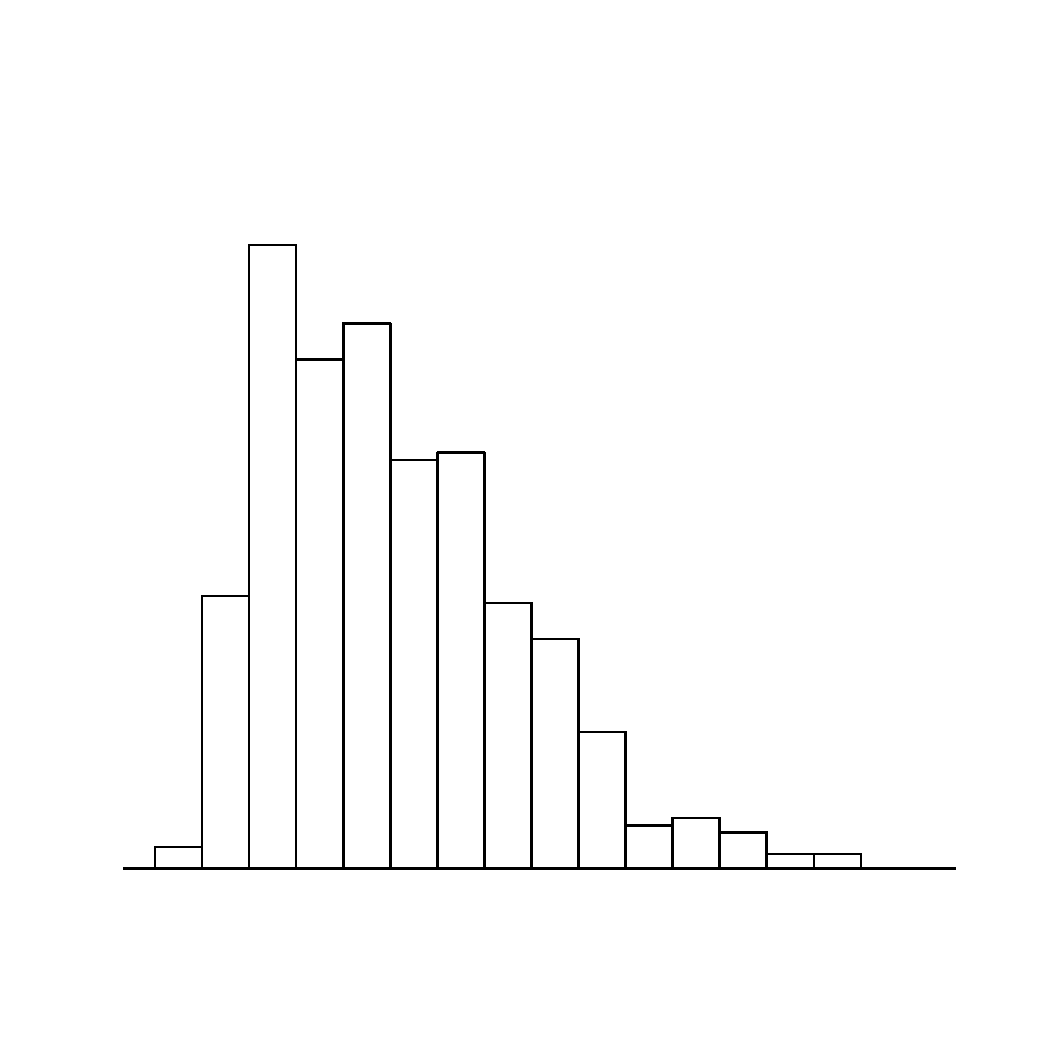
\includegraphics[width=0.32\textwidth]{./images/HistogramShapes_unimodal_skewr.pdf}}
\caption{Histograms for different sets of data each of which exhibit well-known, common characteristics.}
\label{fig:histogram_shapes}
\end{figure}
\end{frame} 

 \begin{frame} 
\begin{figure}[htb]
\centering
\subfigure[\tiny Unimodal (skewed left)]{\label{fig:hist_uni_skewl}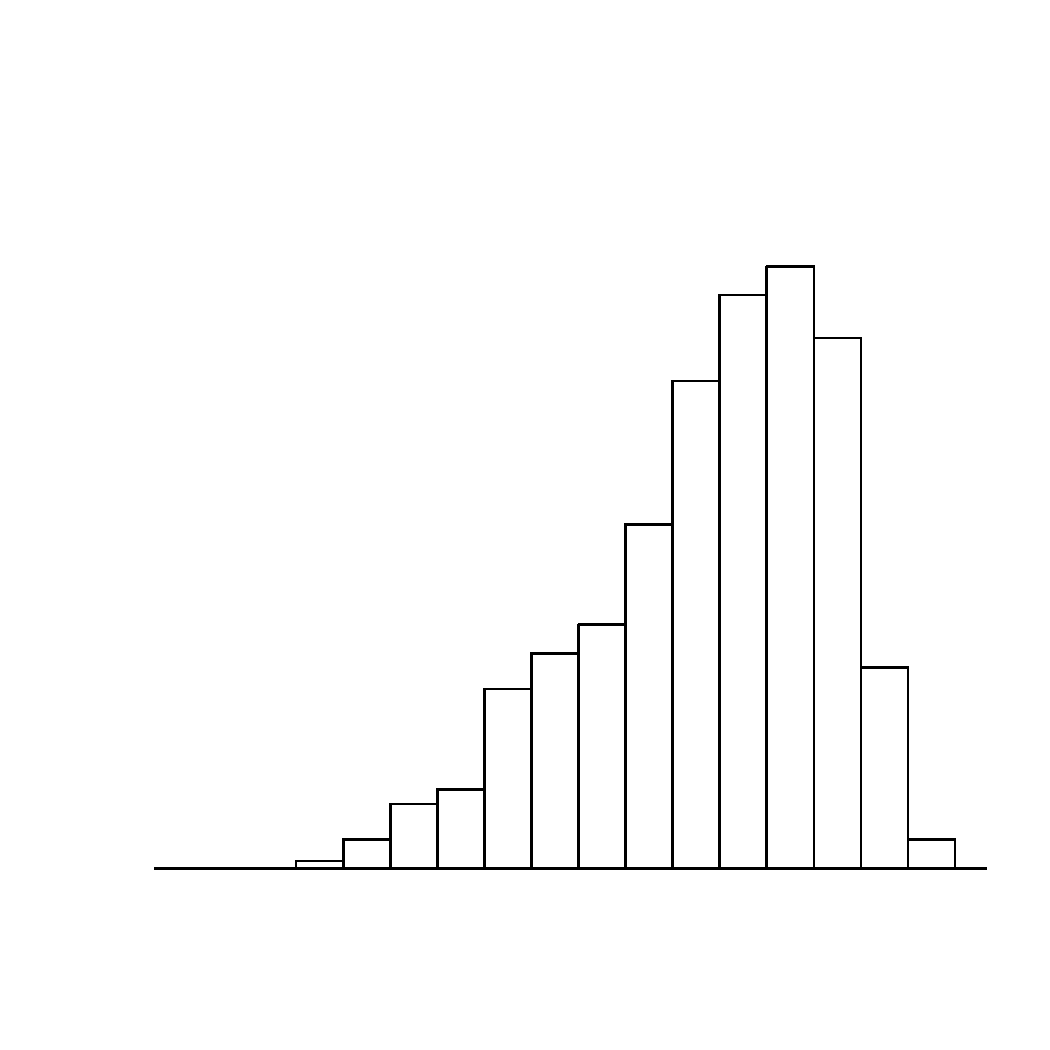
\includegraphics[width=0.32\textwidth]{./images/HistogramShapes_unimodal_skewl.pdf}}
\subfigure[\tiny Exponential]{\label{fig:hist_exp}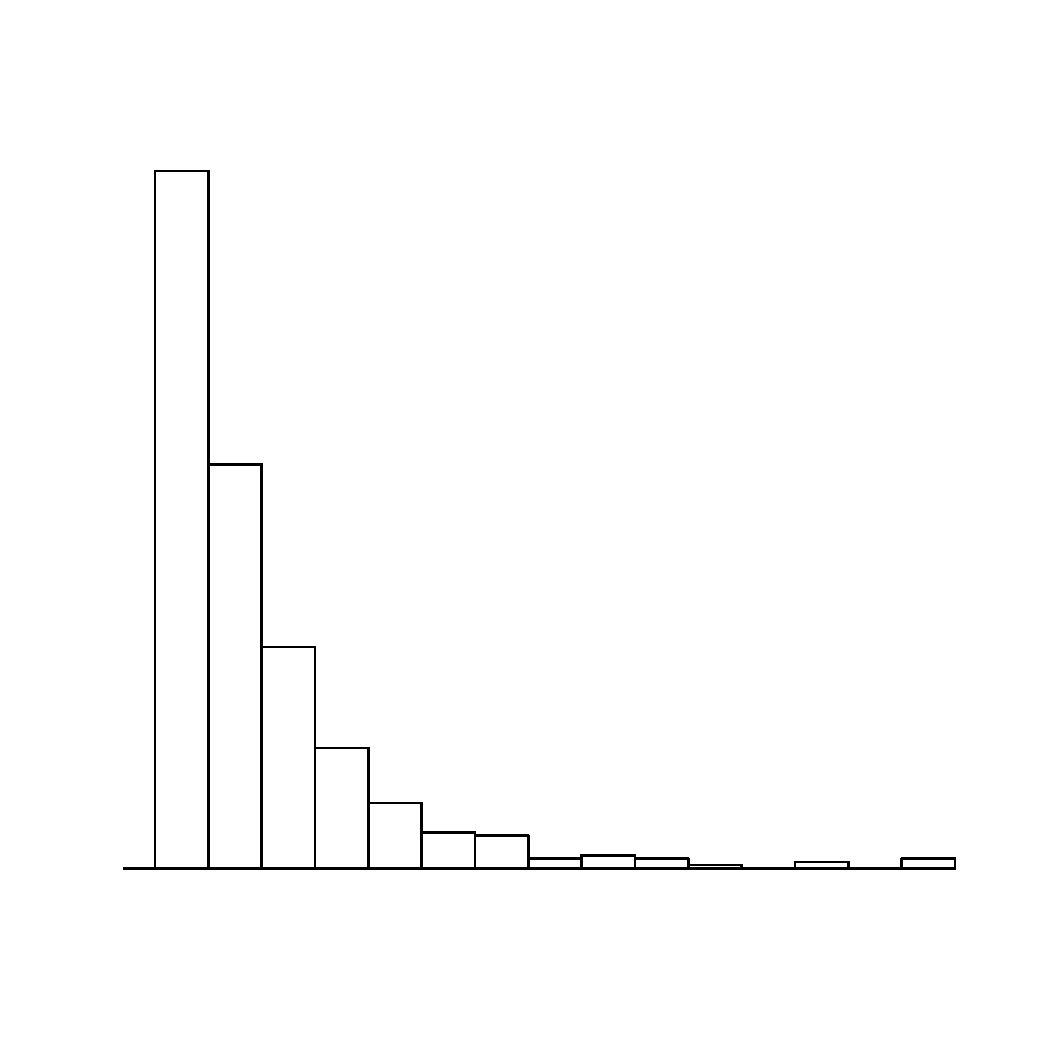
\includegraphics[width=0.32\textwidth]{./images/HistogramShapes_exponential.pdf}}
\subfigure[\tiny Multimodal]{\label{fig:hist_multi}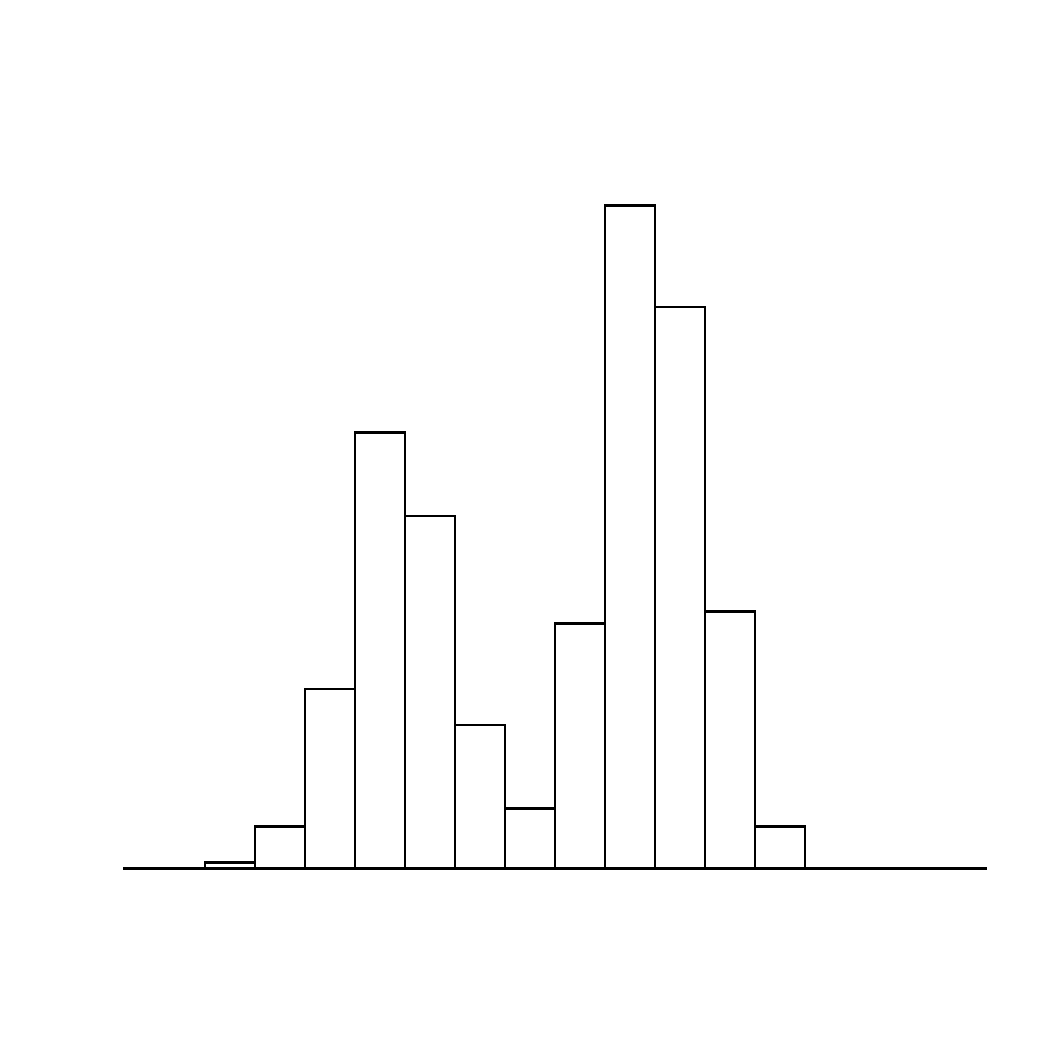
\includegraphics[width=0.32\textwidth]{./images/HistogramShapes_multimodal.pdf}}
\caption{Histograms for different sets of data each of which exhibit well-known, common characteristics.}
\label{fig:histogram_shapes}
\end{figure}
\end{frame} 

\begin{frame} 
	\begin{columns}[t]
		\column{.4\textwidth}
		 
			\centering
			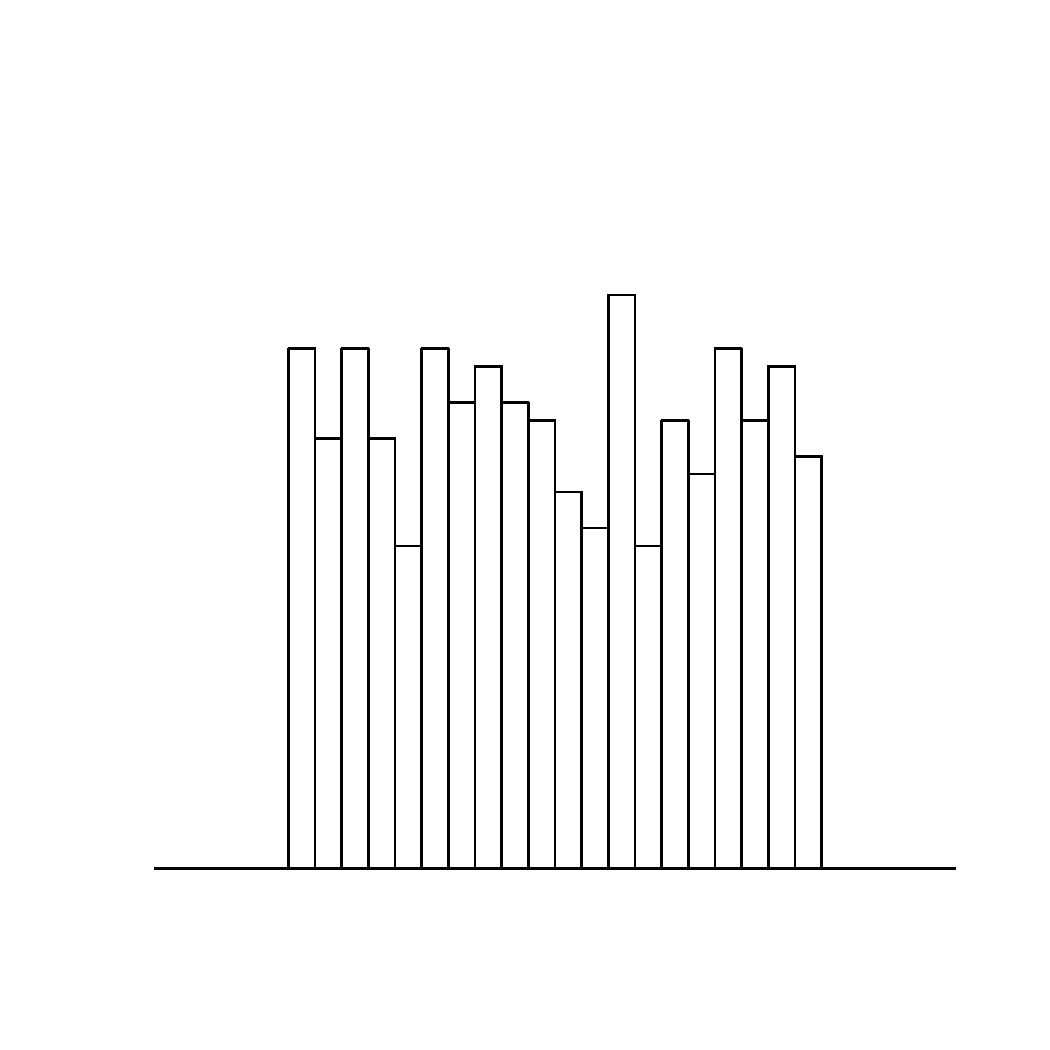
\includegraphics[width=1.0\textwidth]{./images/HistogramShapes_uniform.pdf} \\
			\tiny \textbf{Uniform}

		\column{.6\textwidth} 
		\begin{itemize}
			\item A uniform distribution indicates that a feature is equally likely to take a value in any of the ranges present. 
		\end{itemize}
	\end{columns}
\end{frame} 

\begin{frame} 
	\begin{columns}[t]
		\column{.4\textwidth}
		 
			\centering
			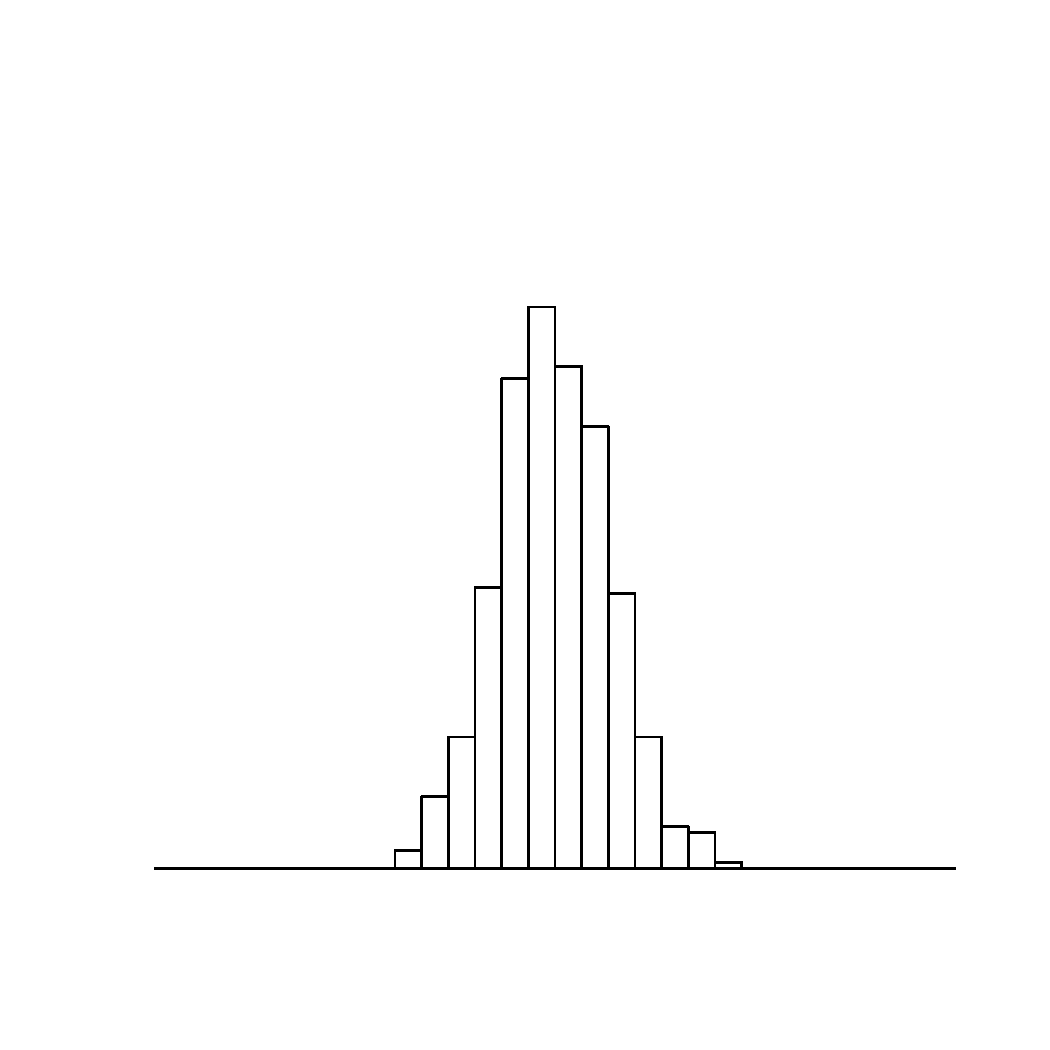
\includegraphics[width=1.0\textwidth]{./images/HistogramShapes_unimodal.pdf}\\
			\tiny \textbf{Normal (Unimodal)}

		\column{.6\textwidth} 
		\begin{itemize}
			\item Features following a normal distribution are characterized by a strong tendency towards a central value and symmetrical variation to either side of this. 
		\end{itemize}
	\end{columns}
\end{frame} 

\begin{frame} 
	\begin{columns}[t]
		\column{.4\textwidth}
		 
			\centering
			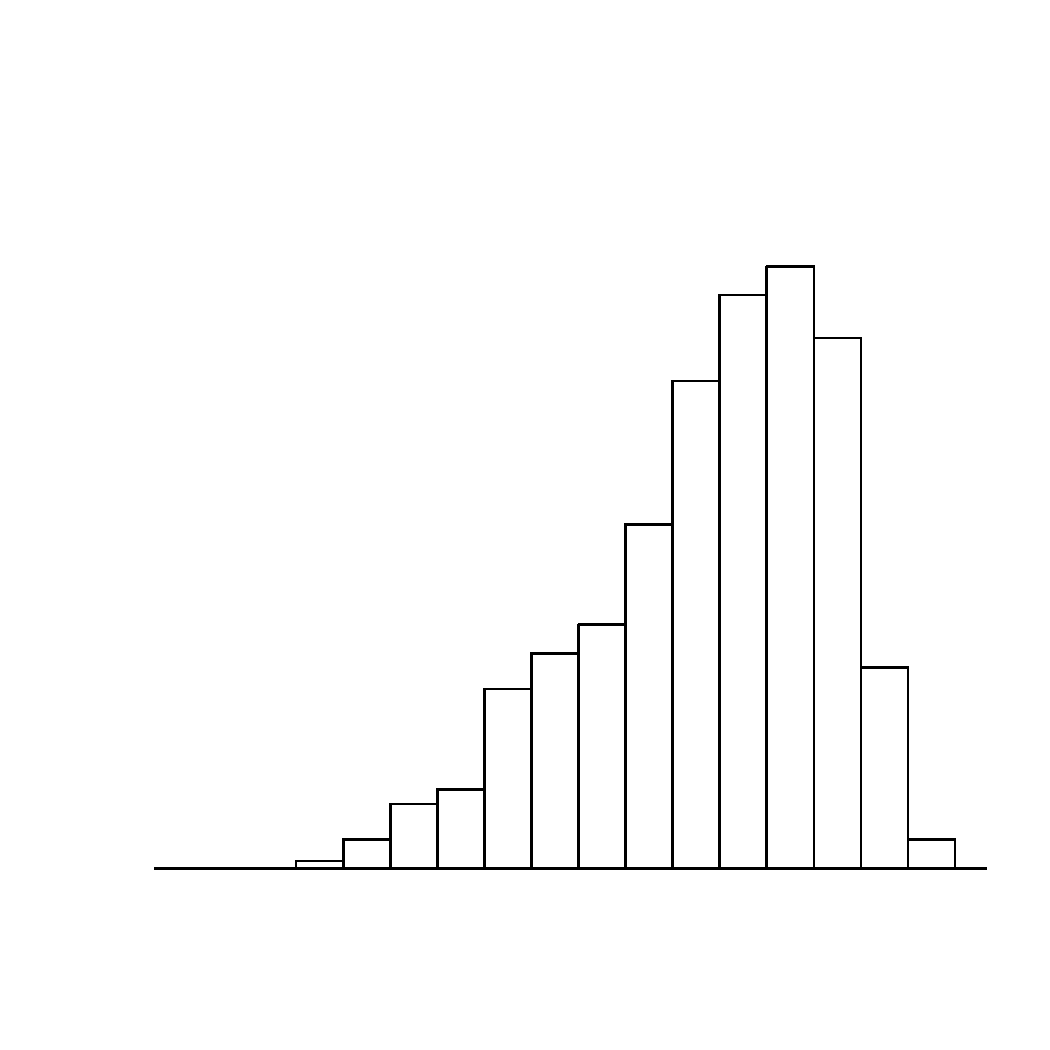
\includegraphics[width=0.8\textwidth]{./images/HistogramShapes_unimodal_skewl.pdf} \\
			\tiny \textbf{Unimodal (skewed left)}
			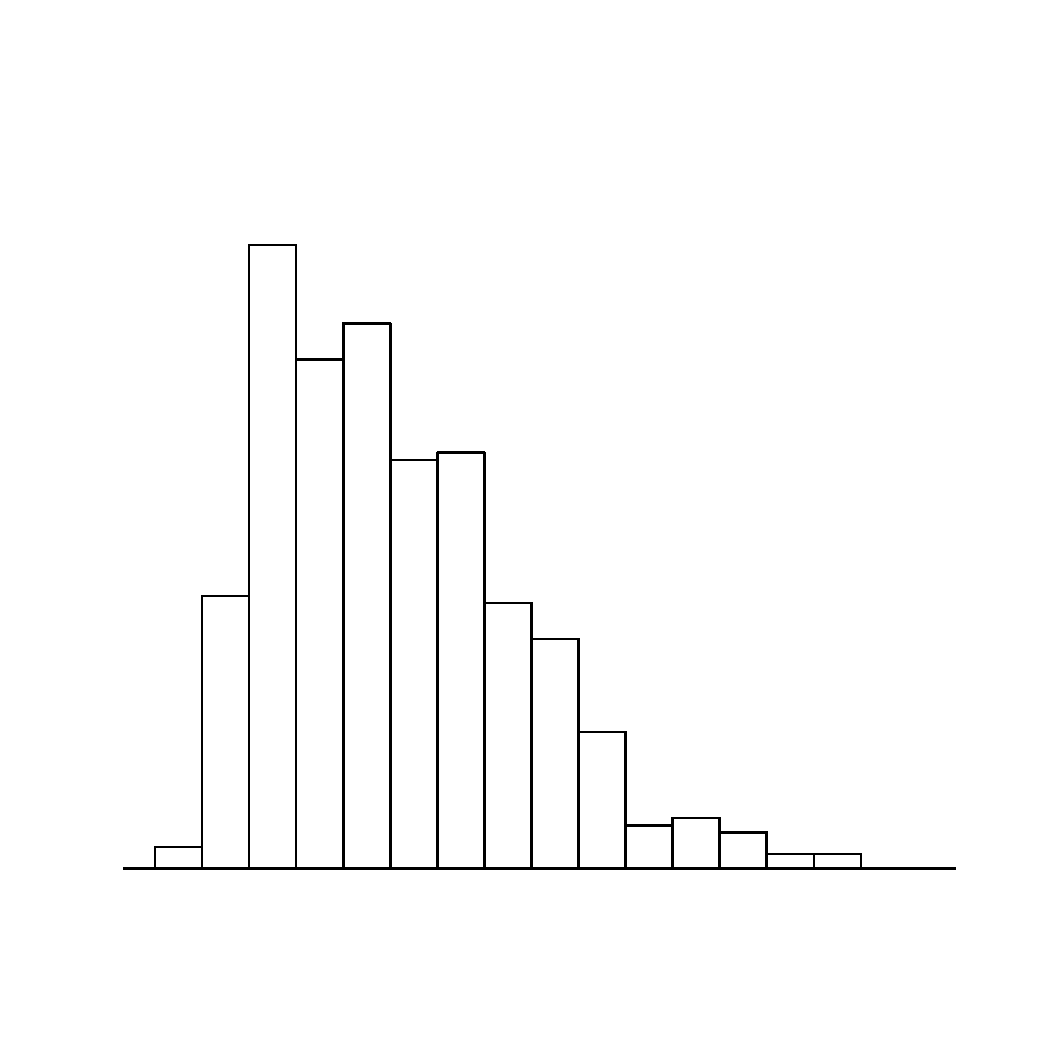
\includegraphics[width=0.8\textwidth]{./images/HistogramShapes_unimodal_skewr.pdf}	\\
			\tiny \textbf{Unimodal (skewed right)}
		
		\column{.6\textwidth} 
		\begin{itemize}
		\item Skew is simply a tendency towards very high (\keyword{right skew}) or very low (keyword{left skew}) values. 
		\end{itemize}
	\end{columns}
\end{frame} 


\begin{frame} 
	\begin{columns}[t]
		\column{.4\textwidth}
		 
			\centering
			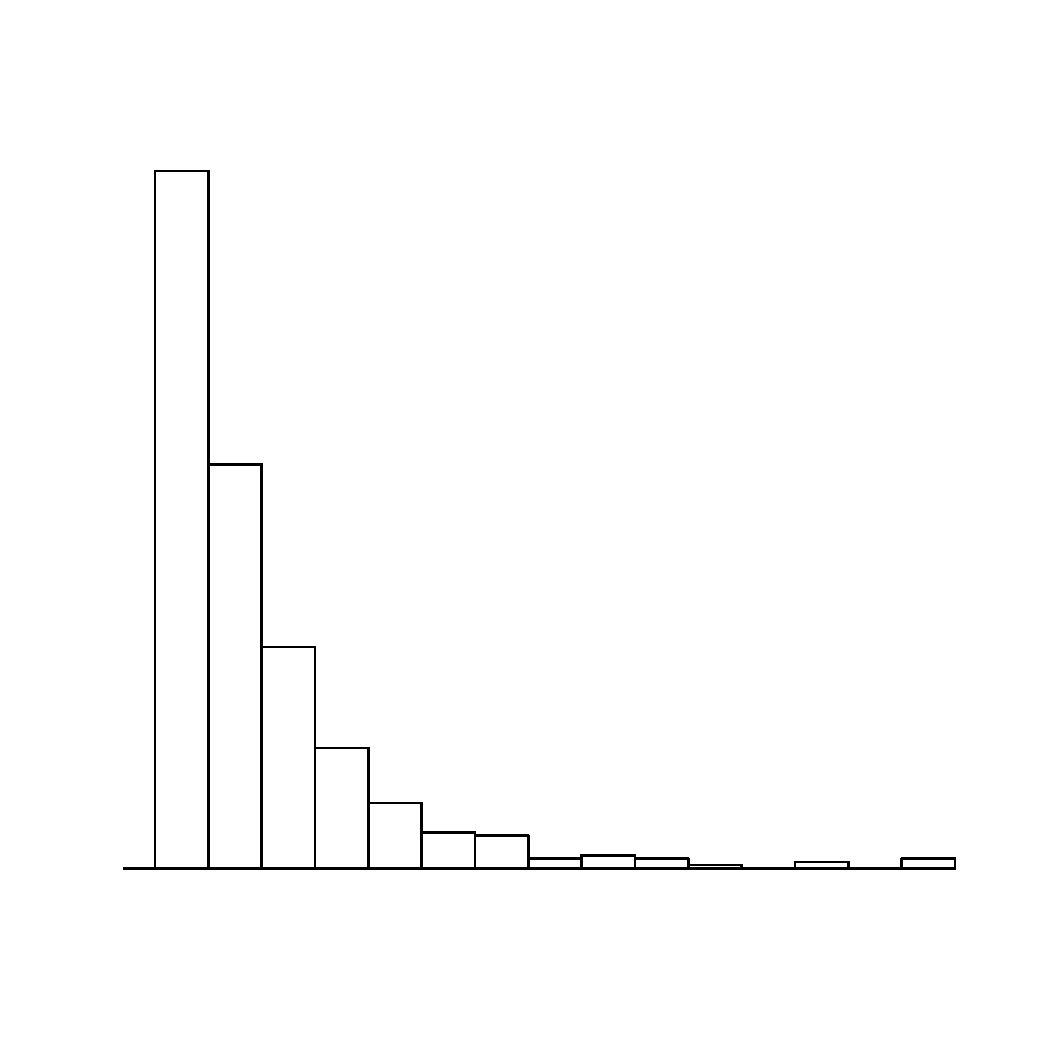
\includegraphics[width=1.0\textwidth]{./images/HistogramShapes_exponential.pdf}\\
			\tiny \textbf{Exponential}

		\column{.6\textwidth} 
		\begin{itemize}
			\item In a feature following an \keyword{exponential distribution} the likelihood of occurrence of a small number of low values is very high, but sharply diminishes as values increase. 
		\end{itemize}
	\end{columns}
\end{frame} 

\begin{frame} 
	\begin{columns}[t]
		\column{.4\textwidth}
		 
			\centering
			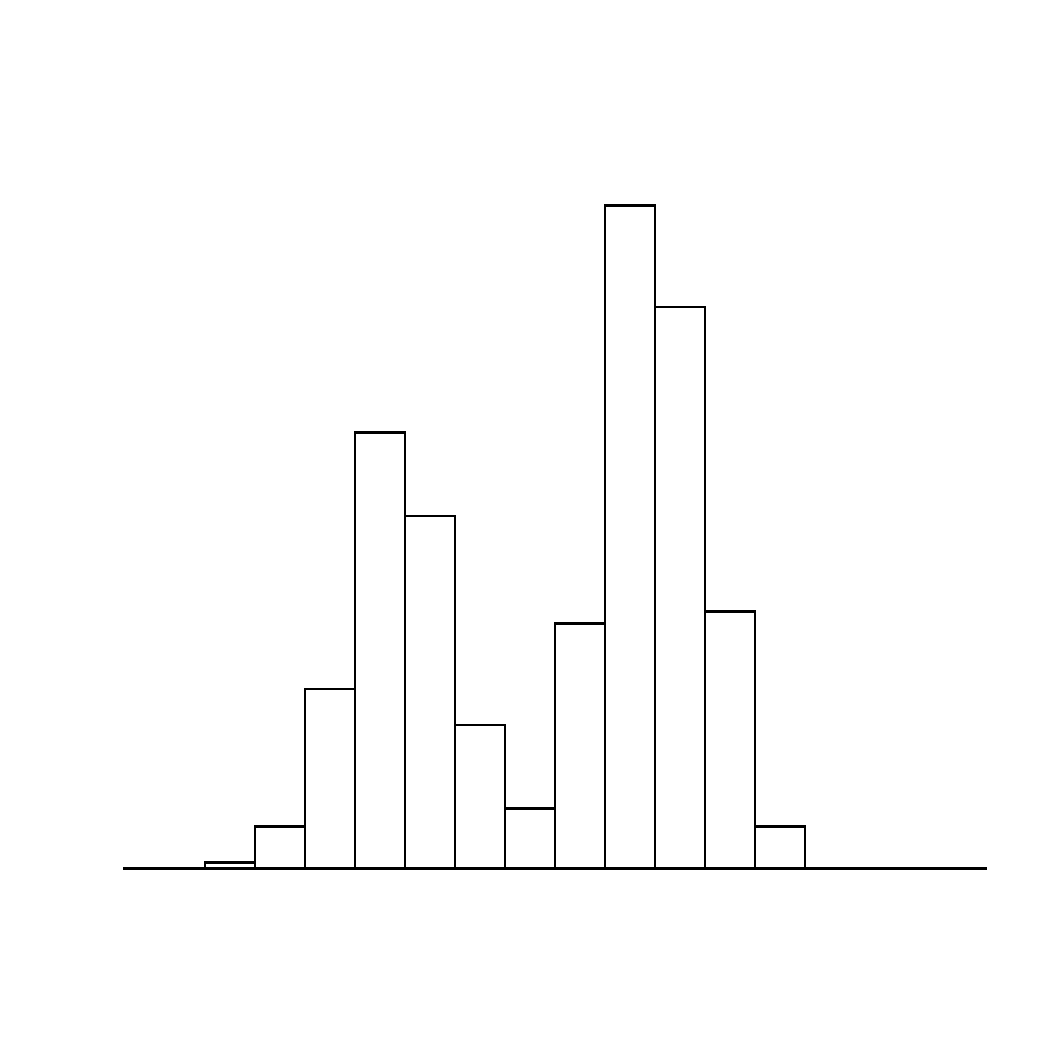
\includegraphics[width=1.0\textwidth]{./images/HistogramShapes_multimodal.pdf}\\
			\tiny \textbf{Multimodal}

		\column{.6\textwidth} 
		\begin{itemize}
			\item A feature characterized by a \keyword{multimodal distribution} has two or more very commonly occurring ranges of values that are clearly separated. 
		\end{itemize}
	\end{columns}
\end{frame} 


 \begin{frame} 
	\begin{itemize}


		\item  The probability density function for the \keyword{normal} distribution (or \keyword{Gaussian distribution}) is
\begin{equation}
\displaystyle N(x, \mu, \sigma) = \frac{1}{\sigma \sqrt{2\pi } }e^{\displaystyle -\frac{ (x-\mu )^2}{2\sigma^2}} 
\label{eq:normal}
\end{equation}
\noindent where $x$ is any value, and $\mu$ and $\sigma$ are parameters that define the shape of the distribution: the \keyword{population mean} and \keyword{population standard deviation}.
	\end{itemize}	
\end{frame} 

 \begin{frame} [plain]
\begin{figure}
\centering
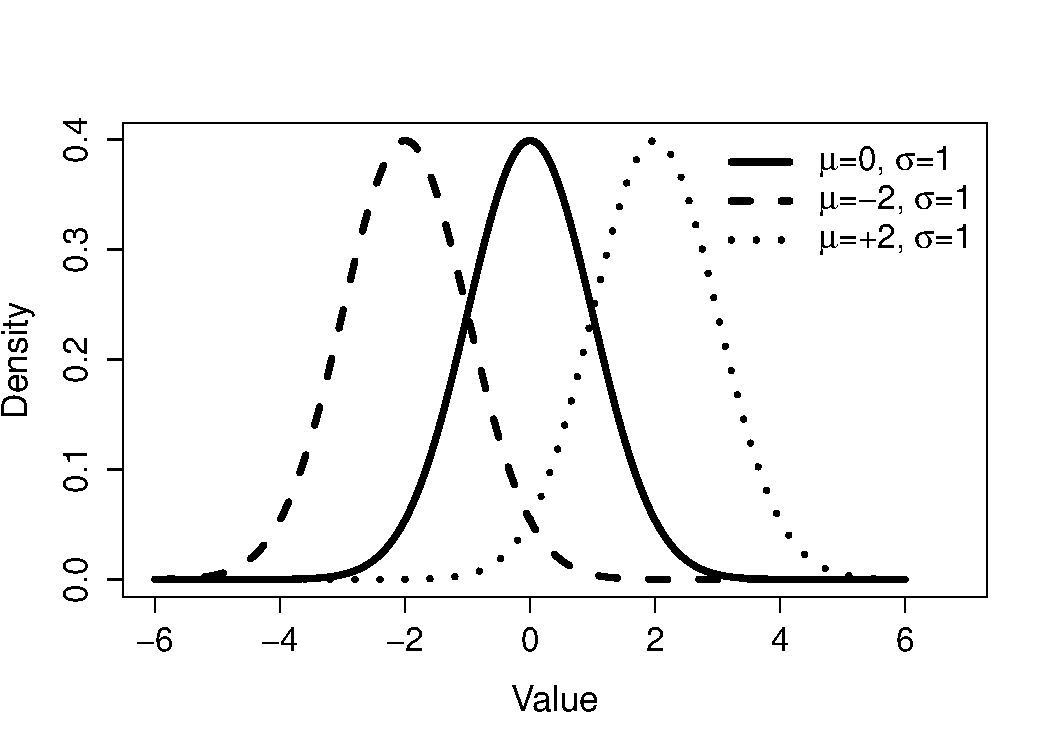
\includegraphics[width=0.85\textwidth]{./images/pdf_NormalParams_mu_short.pdf}
\caption{Three normal distributions with different means but identical standard deviations.}
\label{fig:pdf_normal_means}
\end{figure}
\end{frame} 


 \begin{frame} [plain]
\begin{figure}
\centering
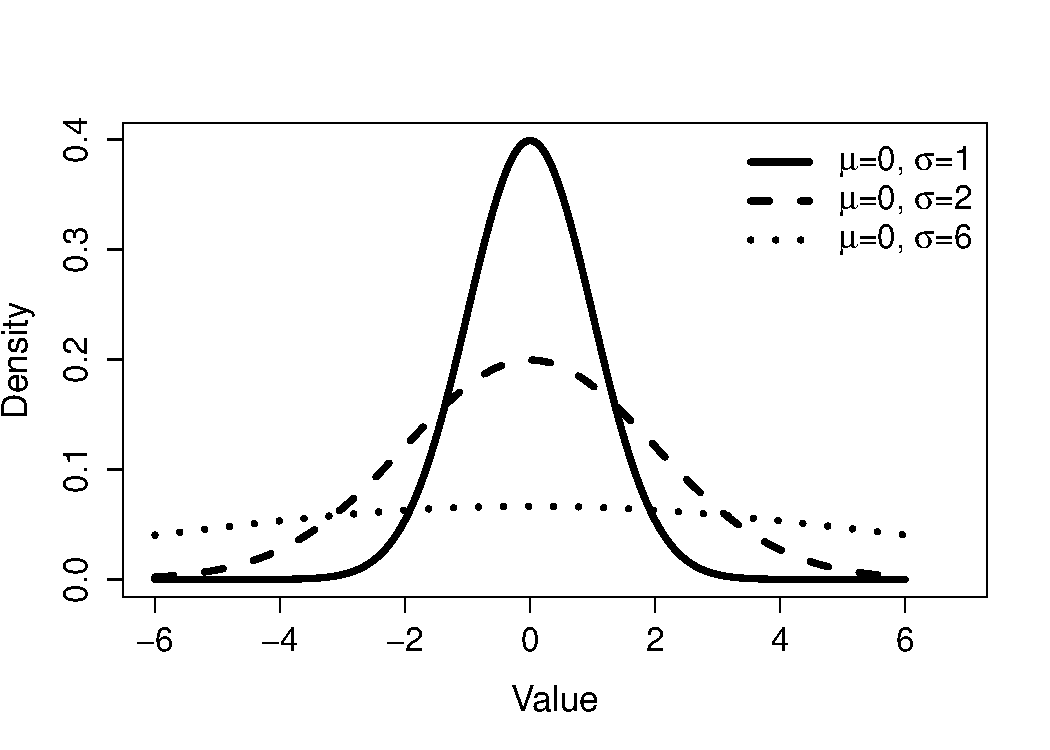
\includegraphics[width=0.85\textwidth]{./images/pdf_NormalParams_sigma_short.pdf}
\caption{Three normal distributions with identical means but different standard deviations.}
\label{fig:pdf_normal_means}
\end{figure}
\end{frame} 

 \begin{frame} 
 	\begin{itemize}
		\item The $68-95-99.7$ rule is a useful characteristic of the normal distribution. 
		\item The rule states that  approximately: 
		 	\begin{itemize}
				\item $68\%$ of the observations will be within one $\sigma$ of $\mu$
				\item $95\%$ of observations will be within two $\sigma$ of $\mu$ 
				\item $99.7\%$ of observations will be within three $\sigma$ of $\mu$. 
		 	\end{itemize}
 	\end{itemize}
\end{frame} 

 \begin{frame} [plain]
\begin{figure}
\centerline{
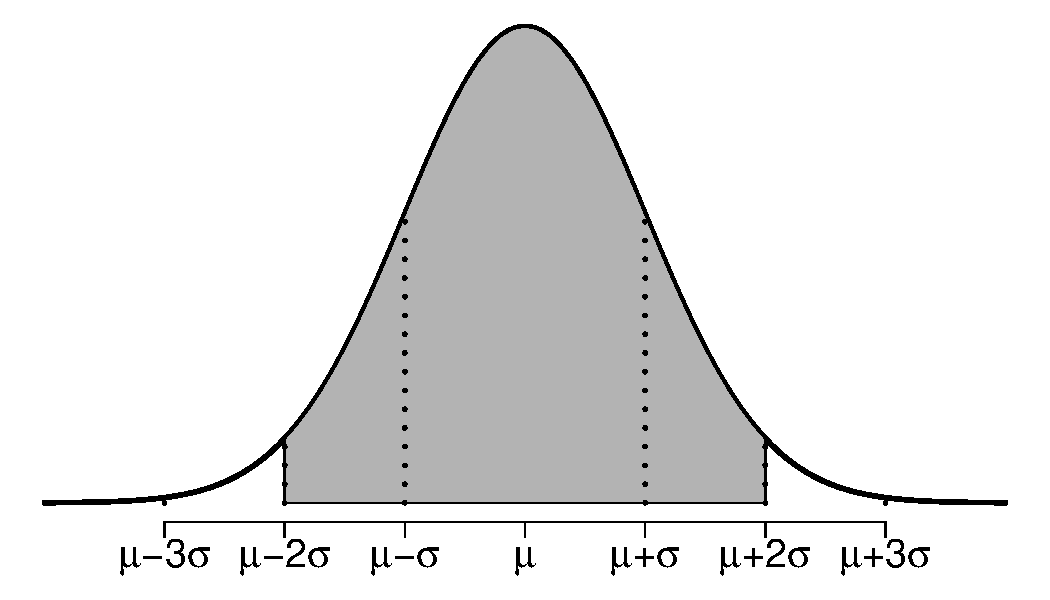
\includegraphics[width=0.55\textwidth]{./images/pdf_normal6895997_shorter.pdf}
}
\caption{An illustration of the $68-95-99.7$ percentage rule that a normal distribution defines as the expected distribution of observations. The grey region defines the area where $95\%$ of observations are expected.}
\label{fig:pdf_normal6895997}
\end{figure}
\end{frame} 

\subsection{Case Study: Motor Insurance Fraud}

\begin{frame}
\begin{block}{Case Study: Motor Insurance Fraud}
Examine the data quality report for the motor insurance fraud prediction scenario and comment on the central tendency and variation of each feature.
\end{block}
\end{frame}


\SectionSlide{Identifying Data Quality Issues}

\begin{frame}
\begin{itemize}
\item A \keyword{data quality issue} is loosely defined as anything \emph{unusual} about the data in an ABT. 
\item The most common data quality issues are: 
\begin{itemize}
\item \keyword{missing values}
\item \keyword{irregular cardinality}
\item \keyword{outliers}
\end{itemize}
\end{itemize}
\end{frame}

\begin{frame}
\begin{itemize}
\item The data quality issues we identify from a data quality report will be of two types: 
\begin{itemize}
\item Data quality issues due to \keyword{invalid data}.
\item Data quality issues due to \keyword{valid data}. 
\end{itemize}
\end{itemize}
\end{frame}


 \begin{frame} 
\begin{table}[tb]
\caption{The structure of a data quality plan.}
\label{tab:dataQualityPlan}
\centering
\begin{footnotesize}
\begin{tabular}{  l  l l }
\hline
Feature	 & Data Quality Issue & Potential Handling Strategies \\
\hline
------ & ------ & ------  \\
------ & ------ & ------  \\
------ & ------ & ------  \\
------ & ------ & ------  \\
\hline
\end{tabular}
\end{footnotesize}
\end{table}
\end{frame} 



\subsection{Case Study: Motor Insurance Fraud}



 \begin{frame} 
\begin{table}[tb]
\caption{The data quality plan for the motor insurance fraud prediction ABT.}
\label{tab:dataQualityPlanCaseStudy}
\centering
\begin{footnotesize}
\begin{tabular}{  l  l l }
\hline
Feature	 & Data Quality Issue & Potential Handling Strategies \\
\hline
\featN{Num Soft Tissue} & Missing values ($2\%$) & ~ \\
 \featN{Claim Amount}  & Outliers (high) &  ~ \\
\featN{Amount Received} & Outliers (high) &  \\
\hline
\end{tabular}
\end{footnotesize}
\end{table}
\end{frame} 


\SectionSlide{Handling Data Quality Issues}

\subsection{Handling Missing Values}


\begin{frame}
\begin{itemize}
\item  Approach 1: Drop any features that have missing value.  
\item Approach 2: Apply \keyword{complete case analysis}. 
\item Approach 3: Derive a \indexkeyword{missing indicator feature} from features with missing value. 
\end{itemize}
\end{frame}

\begin{frame}
\begin{itemize}
\item \keyword{Imputation} replaces missing feature values with a plausible estimated value based on the feature values that are present. 
\item The most common approach to imputation is to replace missing values for a feature with a measure of the central tendency of that feature. 
\item We would be reluctant to use imputation on features missing in excess of $30\%$ of their values and would strongly recommend against the use of imputation on features missing in excess of $50\%$ of their values. 
\end{itemize}
\end{frame}


\subsection{Handling Outliers}



 \begin{frame} 
 \begin{itemize}
 \item The easiest way to handle outliers is to use a \keyword{clamp transformation} that clamps all values above an upper threshold and below a lower threshold to these threshold values, thus removing the offending outliers

\begin{equation}
a_i = 	\begin{cases}
		lower & \text{if } a_i < lower \\
		upper & \text{if } a_i > upper \\
		a_i & otherwise
	\end{cases}
	\label{eqn:clampTransformation}
\end{equation}

where $a_i$ is a specific value of feature $a$, and $lower$ and $upper$ are the lower and upper thresholds. 
\end{itemize}
\end{frame} 


\subsection{Case Study: Motor Insurance Fraud}


\begin{frame}
\begin{block}{Case Study: Motor Insurance Fraud}

What handling strategies would you recommend for the data quality issues found in the motor Insurance fraud ABT?

\end{block}
\end{frame}

 \begin{frame} 
 \begin{block}{Case Study: Motor Insurance Fraud}
\begin{table}[tb]
\caption{The data quality plan for the motor insurance fraud prediction ABT.}
\label{tab:dataQualityPlanCaseStudy2}
\centering
\begin{footnotesize}
\begin{tabular}{  l  l l }
\hline
Feature	 & Data Quality Issue & Potential Handling Strategies \\
\hline
\featN{Num Soft Tissue} & Missing values ($2\%$) & Imputation \\
~ & ~ & (median: 0.0)  \\
 \featN{Claim Amount}  & Outliers (high) &  Clamp transformation \\
 ~ & ~ &  (manual: 0, 80\,000)  \\
\featN{Amount Received} & Outliers (high) & Clamp transformation \\
 ~ & ~ &  (manual: 0, 80\,000)  \\
\hline
\end{tabular}
\end{footnotesize}
\end{table}
\end{block}
\end{frame} 

\SectionSlide{Summary}

\begin{frame} 
\begin{itemize}
\item The key outcomes of the \keyword{data exploration} process are that the practitioner should
\begin{enumerate}
\item Have \emph{gotten to know} the features within the ABT, especially their central tendencies, variations, and \keyword{distributions}.
\item Have identified any \keyword{data quality issues} within the ABT, in particular \keyword{missing values}, \keyword{irregular cardinality}, and \keyword{outliers}.
\item Have corrected any data quality issues due to \keyword{invalid data}.
\item Have recorded any data quality issues due to \keyword{valid data} in a \keyword{data quality plan} along with potential handling strategies.
\item Be confident that enough good quality data exists to continue with a project.
\end{enumerate}  
\end{itemize}
\end{frame} 

\begin{frame}
	\tableofcontents
\end{frame}



\end{document}
